\documentclass[11pt]{article}
\usepackage{natbib}
\usepackage{setspace}
\linespread{1.25}
\usepackage{lmodern}
\usepackage{amssymb,amsmath}
\usepackage{mathtools}
\usepackage[margin=1in]{geometry}
\usepackage{hyperref}
\hypersetup{unicode=true,
	pdftitle={Forecast combination with truncation of the negative weights},
	pdfauthor={Daniel Hsiao},
	pdfborder={0 0 0},
	breaklinks=true}
\urlstyle{same}  % don't use monospace font for urls
\usepackage{graphicx,grffile}
\makeatletter
\def\maxwidth{\ifdim\Gin@nat@width>\linewidth\linewidth\else\Gin@nat@width\fi}
\def\maxheight{\ifdim\Gin@nat@height>\textheight\textheight\else\Gin@nat@height\fi}
\makeatother
%Scale images if necessary, so that they will not overflow the page
%margins by default, and it is still possible to overwrite the defaults
%using explicit options in \includegraphics[width, height, ...]{}
\setkeys{Gin}{width=\maxwidth,height=\maxheight,keepaspectratio}
\setlength{\emergencystretch}{3em}  % prevent overfull lines
\providecommand{\tightlist}{%
	\setlength{\itemsep}{0pt}\setlength{\parskip}{0pt}}
\setcounter{secnumdepth}{5}

\setlength{\parskip}{6pt plus 2pt minus 1pt}
%Use protect on footnotes to avoid problems with footnotes in titles
\let\rmarkdownfootnote\footnote%
\def\footnote{\protect\rmarkdownfootnote}

%Change title format to be more compact
\usepackage{titling}

%Create subtitle command for use in maketitle
\newcommand{\subtitle}[1]{
	\posttitle{
		\begin{center}\large#1\end{center}
	}
}

\setlength{\droptitle}{0em}
\title{Forecast combination with truncation of the negative weights}
\pretitle{\vspace{\droptitle}\centering\huge}
\posttitle{\par}
\author{
	Daniel Hsiao - 382648\\[2.5cm]
	abc}
\preauthor{\centering\large}
\postauthor{\par}
\predate{\centering\large\emph}
\postdate{\par}
\date{November 12, 2018}

\usepackage{placeins}
\usepackage{siunitx}
\usepackage{multirow}
\usepackage{booktabs}

\usepackage{caption}
\captionsetup{font=small}

\begin{document}
	\begin{titlepage}
		\centering
		{\LARGE ERASMUS UNIVERSITY ROTTERDAM}\\[0.5cm]
		{\large Erasmus School of Economics}\\[1.5cm] 
		{\large \textbf{Master Thesis}}\\[0.5cm] 	
		{\LARGE Forecast Combination with Truncation of the Negative Weights}\\[1cm] 
		{\large Ching Teng Hsiao}\\382648\\
		\textit{Quantitative Finance, Erasmus University Rotterdam}\\[1.5cm]
		{\large Supervisor: \\Wendun Wang}\\
		\textit{Econometrics Institute, Erasmus University Rotterdam}\\[ 1cm]
		{\large \today}\\[2.5cm]
		\begin{abstract}
			This thesis examines the predictive power of forecast combinations when the negative weights are not ignored. Instead of removing the negative weights, we use truncation to limit the negative weights to a select range of levels. Using the Survey of Professional Forecasters from the European Central Bank, a dataset with high correlations in forecast errors, this thesis reports a positive performance compared to both equal weights and non-negative weights in five out of six cases. We also show that the truncation is also able to improve the forecast when the selection of the threshold is out-of-sample. Additionally, tests using conditional-bias-adjusted weights, and a simulation study has been carried out to demonstrate the robustness of the method.
		\end{abstract}
	\end{titlepage}
	
	\newpage
	{
		\setcounter{tocdepth}{3}
		\tableofcontents
	}
	\newpage
	
	
	\section{Introduction}\label{introduction}
	We make predictions in almost all of the decisions that we make. Nonetheless, different individuals make different forecasts. The number of unique predictions made increases with a corresponding increase in the number of people making them. Hence, determining which predictions are better and the extent to which group predictions could be better than individual forecasts have always been central issues. When it is not apparent what constitutes the best individual forecast, then most likely there are better solutions that can be developed by using linear combinations of all the predictions that individuals make. A linear combination of all predictions contains the general opinions of the forecasters while lowering the level of idiosyncratic risk. This approach has been fruitful thus far in terms of reducing forecasting errors. In addition, it is essential to review the correlations between different groups of forecasters because they play a vital role in determining the final weights used in prediction.
	
	This study was primarily motivated by the underlying need to improve forecasting accuracy via the determination of optimal weights. Thus far, the optimal combination of forecasts has been overshadowed empirically by the simple averaging method \citep{Bates1969}. Explanations as to why the average performs better in practice than the optimal combination have been centred on the effects of variation and estimation error. In addition, this study was motivated by the overall significance of predictions in our day-to-day undertakings. Each day, people must make decisions based on predictions, e.g., the weather forecast. 
	
	The study will review using the combination of different pairs of forecasts as a way of improving individual forecasts. For instance, the idea of using a combination of forecasts in portfolio optimization with through the use of variance to come up with a weighted average of all the forecasts to improve the ability to construct the forecasts in the first place. This has proven to be successful in decreasing forecasting errors (\cite{Clemen1989}, \cite{Diebold1996}, \cite{Chen1999} , \cite{Dunis2000}, \cite{Stock2004}). Just as in averaging models, taking the median of different forecasts appears to work well \citep{Claeskens2014}.
	
	Furthermore, this study was motivated by suggestions that an estimation involving covariances could be substantial and generally inaccurate. It is important to provide alternative procedures for generating data to increase the estimation error, thus making it large enough to outweigh  the theoretical gains. Further, it is essential to mitigate the estimation error through mitigation techniques. Here, the threshold value comes into play for each forecast to limit the variability. Therefore, the extent to which an optimal combination can be improved using truncation and establishing a coherent understanding of the associated gains are important. Through this study, general results are extended to provide the readers and other beneficiaries of this research with information that could prove helpful in making predictions.
	
	The literature on combining forecasts starts with the seminal article written by \cite{Bates1969}. The literature bloomed, and twenty years later, \cite{Clemen1989} gathered and reviewed over 200 articles included in the literature. Despite the extensive research on forecast combinations, \citeauthor{Clemen1989} found that some issues are still unresolved. One of the issues is: “What is the explanation for the robustness of the simple average of forecasts?” A simple average providing equal weights often outperform more complicated weighting schemes when one compares the combination of point forecasts based on mean squared prediction errors. This result is supported by many studies, for example, \citep{Stock2004}. In 2004, \citeauthor{Elliot2004} published another review of recent theoretical contributions summarizing the developments from \cite{Clemen1989}. Additionally, in research related to this paper, \cite{Gibbs2017} proposed a bias estimation method for adjusting the weight according to the bias.
	
	This paper looks at the correlation between forecasters. The correlation is a factor in weight determination. While many researchers discard correlation due to the uncertainty in the covariance estimation, the effect of the correlation can help the forecast. If both forecasters always overestimate, the high covariance detects this, resulting in a combined forecast that is possible to be not between the two forecasts. Therefore, we wish to examine the effect of negative weights during estimation and to what extent limiting the negative weights can help the forecast combination.
	
	We propose to limit the negative weights instead of neglecting the correlation. We use survey data from the European Central Bank (ECB) to show that the limiting negative weight method can improve the prediction. We impose a threshold parameter, where every negative weight below the threshold is set to zero. Not only does the threshold improve the prediction in terms of mean squared prediction error and mean absolute error, but the threshold method is also able to outperform the equal weight method in some instances.
	
	The result shows that the test statistics\footnote{Lower is better.} decreases in smooth adjustments, and the choice of threshold parameter is not very sensitive to minor changes. This lack of sensitivity means that one does not need to worry about the error during threshold selection overly much, as choosing a slightly incorrect threshold does not impact the performance substantially. We show that even when using in-sample threshold parameter selection, the threshold method still outperforms the equal weight method.
	
	We look further into bias correction and simulation. Bias correction aims to decrease the weights of the forecasts with known bias, while, in the simulation study, we show the effect of noise-to-signal ratios and correlations on the shape of the mean squared prediction error against threshold values. Bias estimation does not improve forecasting in most cases, but it does improve one time series significantly in a case where thresholds do not help. The simulation, on the other hand, shows that when the correlation increases, the MSPE in the end position at the threshold of zero decreases. A similar effect can be found in the noise-to-signal ratio. When the noise-to-signal ratio increases, the MSPE achievable through negative weights increases.
	
	The paper is structured as follows: Section 2 starts with methodology and the implications for truncation. Section 3 explains the data structure and the preliminary analysis of the data. Section 4 provides empirical results and a simulation study of the threshold method involving signal-to-noise ratios and correlations.
	
	
	\section{Methodology}\label{methodology}
	
	\subsection{Standard Approach with High Covariance}\label{standard-approach}
	
	In this paper, we consider the two-variable case for illustrative purposes. We have
	two forecasts, \(y_1\) and \(y_2\), of the true variable \(y\). We want
	to combine \(y_1\) and \(y_2\) with a weight \(w\) such that 
	\(y_c = w y_1 + (1-w) y_2\). Assuming that these forecasts follow some distribution with a finite first and second moment, e.g.,
	\(y_1 \sim D(0,\sigma_1)\), \(y_2 \sim D(0,\sigma_2)\), and
	\(corr(y_1,y_2)=\rho\), then the variance of the combined forecast
	\(y_c\) is
	\begin{equation}
	\label{eqn: var yc}
	Var(y_c) = w^2\sigma_1^2+ (1-w)^2\sigma_2^2+2w(1-w)\sigma_1\sigma_2\rho,
	\end{equation}
	and the optimal weight with minimum variance is
	\begin{equation}
	\label{eqn: simple weight}
	w^*=\frac{\sigma_2^2-\sigma_1\sigma_2\rho}{\sigma_1^2+\sigma_2^2 -2\sigma_1\sigma_2\rho}.
	\end{equation}
	Equation \ref{eqn: simple weight} is the standard approach in
	combination theory, and it is in this area that extensive research has been done. We refer to this weight as the optimal weight. Some empirical results on Equation \ref{eqn: simple weight} argue against this approach. Two common
	alternative solutions are based on a diagonal covariance matrix and equal weights.
	
	Ignoring the correlation term \(\rho\) by setting \(\rho=0\), we obtain the
	inverse relation for the variance
	\begin{equation}
	\label{eqn: simple weight no corr}
	w=\frac{\sigma_2^2}{\sigma_1^2+\sigma_2^2}.
	\end{equation}
	This is a robust way of avoiding the estimation of the covariance as the
	dimension increases. The number of parameters needed to estimate a
	covariance with dimension \(n\) is \(\frac{1}{2}n(n+1)\), which is
	quadratic in \(n\). When the variances are estimated instead, the
	number of parameters to be estimated reduces to \(n\), which 
	decreases the estimation error greatly \citep{Stock2001}.
	
	Applying an additional restriction by setting $\sigma_1=\sigma_2$, we obtain equal weights. Applying equal weights is another common approach that works better than optimal weights empirically \citep{Clemen1989} in terms of forecast error. In this case, the forecast combination reduces to the
	arithmetic mean of all forecasts. Hence, when using equal weights, there is no need to estimate the weights.
	Estimating the weights for the optimal weights method increases or shifts the forecasting errors due to the
	additional estimation error made in estimating \(w\). This estimation error then has a negative effect on the forecast. 
	
	Looking back to Equation \ref{eqn: simple weight}, we examine the effect
	of a high correlation term. Assuming without loss of generality that
	\(\sigma_1 =\sigma_2 (1 + \delta)\), where \(\delta>0\), we rewrite the optimal
	weight as
	\begin{equation}
	\label{eqn: w high corr}
	w^* = \frac{(-\rho\delta+ (1-\rho))}{2(1-\rho - (1-\rho)\delta)+\delta^2}.
	\end{equation}
	The numerator for \(w\) consists of a weighted
	mean between $-\delta$ and $1$ with weights \(\rho\) and $1-\rho$, respectively. When \(\rho\)
	is small, the weight is close to the value in Equation
	\ref{eqn: simple weight no corr}, which is $\frac{1}{1+(1+\delta)^2}$. When \(\rho\) is large, the negative in the numerator, \(-\delta\), dominates and results in a negative
	weight, i.e.,  the weight approaches
	\begin{equation}
	\label{eqn: w simple rho 1}
	w^* = \frac{-\delta}{\delta^2}
	\end{equation}
	as $\rho$ approaches 1. As $\delta$ approaches 0, the weight quickly approaches $-\infty$. This result is contrary to the intuition involved in equal weights, where the variances are equal.
	Only when $\delta >1$, i.e., $\sigma_1 > 2\sigma_2$, will the weight be above -1.
	The boundary case is
	\begin{equation}
	\label{eqn: corr boundary}
	\rho = \frac{\sigma_2}{\sigma_1},
	\end{equation}
	which \(w\) decreases to \(0\), and \(y_c = y_2\).
	
	\subsection{\texorpdfstring{With estimation error of
			\(w\)}{Including the estimation error for w}}\label{including-the-estimation-error-of-w}
	
	We can also consider the optimal weight to be non-deterministic but related to
	\(y\), e.g., in a trivariate distribution with finite third and fourth
	moments \citep{Claeskens2014}. Under a trivariate distribution, the variance of the weight
	influences the expected value and the variance of the combined forecast.
	The expected value and the variance of the combined forecast become
	\begin{equation}
	\label{eqn: E var yc w/ var w}
	\begin{aligned}
	E(y_c) =& \mu + (cov(w, y_1-y_2))^2\\
	var(y_c) =& E(w)^2\sigma_1^2 + (1-E(w))^2\sigma_2^2 + 2E(w)(1-E(w))\rho\sigma_1\sigma_2 \\
	+& E[(w-E(w))(y_1-y_2) (E(w)y_1 + (1-E(w))y_2 - \mu)] \\
	+& E[(w-E(w))^2 (y_1-y_2)^2] - cov(w,y_1-y_2)^2.
	\end{aligned}
	\end{equation}
	Equation \ref{eqn: E var yc w/ var w} shows the general case for the
	combined forecast. If the covariance between \(w\) and \(y_1-y_2\) is
	not \(0\), the combined forecast will be biased, with bias
	\(cov(w, y_1-y_2)^2\). The variance also increases from equation
	\ref{eqn: var yc} by
	\(E[(w-E(w))(y_1-y_2) (E(w)y_1 + (1-E(w))y_2 - \mu)]+E[(w-E(w))^2 (y_1-y_2)^2] - cov(w,y_1-y_2)^2\).
	The only requirements for this case are that the individual forecasts must be
	unbiased and that the weights sum to 1.
	
	Let \(d = (d_1, d_2)'\) be the third moment between \(y_1\), \(y_2\), and $w$,
	and let
	\(\begin{bmatrix} \sigma_{11} & \sigma_{12}\\ \sigma_{12} & \sigma_{22}\end{bmatrix}\)
	be the (co)variance matrix of $(y_1,y_2)$. Then we have
	\begin{equation}
	\label{eqn: w w/ var w}
	\begin{aligned}
	w^\dagger = w^*(1+\frac{\sigma_{22} d_1 + \sigma_{11} d_2 -\sigma_{12} (d_1 + d_2)}{\sigma_{11}\sigma_{22} - \sigma_{12}^2}) - \frac{\sigma_{22} d_1 - \sigma_{12}d_2}{\sigma_{11}\sigma_{22} - \sigma_{12}^2}.
	\end{aligned}
	\end{equation}
	The non-deterministic weight is then a linear combination involving the
	original weight. The non-deterministic weight does not change if the
	third moment is \(0\). 
	When considering real life, it is not hard to imagine that the weights are correlated with the data used to calculate the weights. However, since the weights are unobserved, there are no straightforward methods for finding the third moment.
	
	Now, we look at the scaling parameter and the intercept adjustment vector in Equation \ref{eqn: w w/ var w}. Under same conditions, I,e, where
	\(\sigma_1 =\sigma_2 (1 + \delta)\), we rewrite the determinant as
	\begin{equation}
	\sigma_{11}\sigma_{22} - \sigma_{12}^2 = \sigma_{22}\sigma_{11} (1- \rho^2),
	\end{equation}
	and the weight becomes
	\begin{equation}
	\label{eqn: scaling factors}
	\begin{aligned}
	w^\dagger = w^*(1+\frac{d_1(1- \rho(1+\delta)) + d_2 ((1+\delta)^2-\rho(1+\delta))} {\sigma_{11} (1- \rho^2)}) - \frac{d_1-\rho(1+\delta) d_2}{\sigma_{11}(1- \rho^2)}.
	\end{aligned}
	\end{equation}
	In the special case in which $\sigma_{22} d_1 - \sigma_{12}d_2=0$, we get $d_1=\rho(1+\delta) d_2$ and 
	\begin{equation}
	\label{eqn: special case}
	\begin{aligned}
	w^\dagger = w^*(1+\frac{d_2} {\sigma_{22}}).
	\end{aligned}
	\end{equation}
	The direction of the weight bias is only dependent on the sign of $d_2$. If $d_2$ is large, $w^\dagger$ becomes large, and vice versa. The correlation no longer plays a role in the bias associated with $w^\dagger$.
	
	The behaviour of $w^\dagger$ when the correlation is close to 0 or 1 is also of interest. When $\rho$ is 0, equation \ref{eqn: scaling factors} simplifies to 
	\begin{equation}
	\label{eqn: scaling factor rho 0}
	\begin{aligned}
	w^\dagger &= w^*(1+\frac{d_1 + d_2 (1+\delta)^2} {\sigma_{11} }) - \frac{d_1}{\sigma_{11}}\\
	&=w^* +w^*(\frac{d_2}{\sigma_{22} }) + (1-w^*)(-\frac{d_1}{\sigma_{11}}).
	\end{aligned}
	\end{equation}
	The bias for $w^\dagger$ is now a weighted average between $\frac{d_1}{\sigma_{11}}$ and $\frac{d_2}{\sigma_{22}}$ using the weight $w^*$ itself. We arrive at the same special case described by Equation \ref{eqn: special case} when $d_1=0$.
	
	When $\rho$ reaches 1, the determinant becomes 0, and the limit of the weight becomes $\infty$ or $-\infty$, depending on the signs of $d_1$ and $d_2$. Due to the fact that the sign of the third moment between $w$ and $y$ is unknown, we cannot infer the sign of the scaling factor. Compared to Equation \ref{eqn: w simple rho 1}, where the effect of not knowing the sign of $\delta$ is limited as long as $\delta$ is large enough, the weight in Equation \ref{eqn: w w/ var w} is unrestricted and can take any value. This fact has a negative effect on the estimation, as the increase in $\rho$ increases the estimation's uncertainty.
	
	\subsection{Truncated weight}\label{truncated-weight}
	
	To avoid highly correlated forecasts, truncation is used on the
	weights after estimation. Given the optimal weight $w^*$, the truncated weight is 
	\begin{equation}
	\label{eqn: w trunc}
	\tilde{w} = 
	\begin{dcases}
	w^* &, \text{ if } c\leq w^*\leq 1-c \\
	c &, \text{ if } w^*<c \\
	1-c &, \text{ if } w^*>1-c.
	\end{dcases}
	\end{equation}
	
	This weight estimation limits the minimum weight to $c$ and normalises the sum of the weights to $1$. 
	
	Due to the truncation, the bias and variance change with respect to the choice of $c$. Assume that the weight $w$ follows the probability density function $D(w)$ and the truncation threshold is negative $c<0$. Then the bias of the estimation can be expressed as
	\begin{equation}
	\label{eqn: bias trunc}
	\begin{aligned}
	Bias(\tilde{w}) &= \int_{-\infty}^{c} (w-c) D(w)dw + (1-\frac{1}{\alpha})\int_{c}^{\infty}( w-E(w))D(w)dw\\
	\alpha &= \int_{c}^{\infty} w dw\\
	&\geq \int_{-\infty}^{\infty} w dw\\
	&=1.
	\end{aligned}
	\end{equation}
	The bias is the sum of the bias from the truncated weights and the bias from the rescaling. When the threshold goes to $-\infty$, both quantities in the sum go to $0$, meaning that the bias goes to $0$.
	
	The variance of the truncated weight is
	\begin{equation}
	\label{eqn: var trunc}
	\begin{aligned}
	Var(\tilde{w}) &= \frac{1}{\alpha^2} \int_{c}^{\infty} (w-E(w))^2 D(w) dw\\
	&\leq \int_{c}^{\infty} (w-E(w))^2 D(w) dw\\
	&\leq \int_{-\infty}^{\infty} (w-E(w))^2 D(w) dw\\
	&=Var(w^*)
	\end{aligned}
	\end{equation}
	Since $\alpha \geq 1$,  scaling decreases the variance. Since $(w-E(W))^2 \geq 0$, setting the truncation and rescaling results in the variance of the truncated weight being smaller than that of the original weight. The variance should be considered in terms of its relation to $c$. When the threshold becomes small; $c \rightarrow -\infty$; the effect of the threshold disappears; the two variances become equal, i.e., $Var(\tilde{w}) = Var(w^*)$; and $\alpha = 1$.
	
	Increasing the threshold $c$ increases the bias in the estimation but also decreases the variance. The case in which the mean squared error (MSE) is at a minimum is, therefore, the most interesting. Due to the unknown distribution of the weights, the minimum MSE needs to be computed numerically.
	
	One special case involving $c$ is worth noting. When $c$ is set to $0$, using a truncated weight becomes equivalent to using a variable selection method. If the weight falls below the threshold, the forecast is discarded. Setting $c$ to $0$, however, does not imply the reduction of Equations \ref{eqn: bias trunc} and \ref{eqn: var trunc}.
	
	Another special case occurs when there is an assumption made concerning the distribution of the weights. If the weights follow a normal distribution, $w\sim N(\mu,\sigma)$, where $\phi(x)$ and $\Phi(x)$ are the probability density function and cumulative density function of standard normal distribution, respectively, then the bias and the variance are 
	\begin{equation}
	\label{eqn: trunc norm}
	\begin{aligned}
	Bias(\tilde(w)) &= \sigma \frac{\phi(c)}{1-\Phi(c)}\\
	Var(\tilde(w)) &= \sigma^2 \bigg[1-\frac{c\phi(c)}{1-\Phi(c)}-\big(\frac{\phi(c)}{1-\Phi(c)}\big)^2\bigg].
	\end{aligned}
	\end{equation}
	The effect of $c$ reaching $-\infty$ is the same as in Equations \ref{eqn: bias trunc} and \ref{eqn: var trunc}, i.e., the bias becomes $0$ and variance becomes the variance of the original weight. The effect of the squared bias and the variance on the MSE is
	\begin{equation}
	\label{eqn: trunc mse}
	MSE(\tilde{w}) = \sigma^2 \bigg[ 1 -\frac{c\phi(c)}{1-\Phi(c)}\bigg].
	\end{equation}
	Since the MSE of the optimal weight is the variance, i.e., $MSE(w^*) = \sigma^2$, the derivative of the difference in the MSE is
	\begin{equation}
	\frac{\partial \triangle MSE}{\partial c} = \sigma^2\frac{\bigg[(1-c^2)\phi(c)[1-\Phi(c)]+c\phi(c)^2\bigg]}{(1-\Phi(c))^2}.
	\end{equation}
	Numerical optimisation shows that the maximum $\triangle MSE$ is reached at $c=-0.84\sigma^2$. However, as the true $\sigma^2$ is unknown, this optimisation does not translate into analytical results.
	
	\subsection{Bias Correction}\label{bias-correction}
	In this section, we provide the bias correction by following \cite{Gibbs2017}, who suggest that knowing the conditional bias helps in terms of weight estimation. If the conditional bias is large for a certain forecast, the forecast should be under-weighted, similar to the case in which the variance of the forecast is large.
	
	To begin bias estimation, let the prediction error from forecast \(i\) be \(\epsilon_i = y - y_i\). Then we can decompose the prediction error into a predictable term and an unpredictable term
	
	\begin{equation}
	\label{eqn: w bias assumption}
	\epsilon_i = b_i + \xi_i. 
	\end{equation}
	with expected value
	\begin{equation}
	\label{eqn: bias estimate}
	E(\epsilon_i) = b_i.
	\end{equation}
	
	Let $b_i \neq 0$, then the expected combined error is non-zero
	\begin{equation}
	E(\epsilon_c) = wb_1+(1-w)b_2
	\end{equation}
	and the variance is
	\begin{equation}
	Var(\epsilon_c) = w^2\sigma_{\xi,11} + (1-w)^2\sigma_{\xi,22} + 2w(1-w)\rho_{\xi_1,\xi_2}\sigma_{\xi,1}\sigma_{\xi,2}
	\end{equation},
	where $\sigma_{\xi_i}$ is the variance of $\xi_i$.
	
	Since the expected value is non-zero, we can minimise the MSE to calculate the weight.
	With \(b_{ij}=b_i*b_j\), minimising the mean squared error leads to
	\begin{equation}
	\label{eqn: w bias}
	\begin{aligned}
	\hat{w} &= \frac{\sigma_{\xi,22}-\sigma_{\xi,12}+b_{22}-b_{12}}{\sigma_{\xi,11}+\sigma_{\xi,22}-2\sigma_{\xi,12}+b_{11}+b_{22}-2b_{12}}.
	\end{aligned}
	\end{equation}
	Notice that for Equation \ref{eqn: w bias}, we can use Equation \ref{eqn: simple weight}'s optimal weight $w^*$ with a slight modification to the variance matrix, i.e., we can replace the original matrix with
	\(\begin{bmatrix}\sigma_{\xi,11}+b_{11} & \sigma_{\xi,12}+b_{12}\\ \sigma_{\xi,12}+b_{12} & \sigma_{\xi,22}+b_{22}\end{bmatrix}\), and the results will be the same.
	
	We study a few special cases here. When the biases are equal, i.e., $b_1=b_2$, we have $\hat{w}=w^*$. In this case, the biases cancel each other out. 
	
	If $\rho_{\xi_1,\xi_2}=0$ and $b_1=0$, we have
	\begin{equation}
	\begin{aligned}
	\hat{w} &= \frac{\sigma_{\xi,22}+b_{22}}{\sigma_{\xi,11}+\sigma_{\xi,22}+b_{22}}
	\end{aligned}
	\end{equation},
	which converges to 1 if $b_2 \to \infty$.
	
	When $\rho_{\xi_1,\xi_2}=0$ and $b_2=0$, we have
	\begin{equation}
	\begin{aligned}
	\hat{w} &= \frac{\sigma_{\xi,22}}{\sigma_{\xi,11}+\sigma_{\xi,22}+b_{11}}
	\end{aligned}
	\end{equation},
	which converges to 0 if $b_1 \to \infty$. Here, we see that the effect of the bias is similar to that of the variance. The higher the bias, the lower the weight of the forecast.
	
	The final special case involves $\rho_{\xi_1,\xi_2}=0$. Then we have
	\begin{equation}
	\begin{aligned}
	\hat{w} &= \frac{\sigma_{\xi,22}+b_{22}-b_{12}}{\sigma_{\xi,11}+\sigma_{\xi,22}+b_{11}+b_{22}-2b_{12}}.
	\end{aligned}
	\end{equation}
	An approach similar to that used in Equation \ref{eqn: w high corr} is used here, with $b_1 = b_2 (1+\gamma)$. However, $b_{22}$ cannot be cancelled out. We now have
	\begin{equation}
	\begin{aligned}
	\hat{w} &= \frac{\sigma_{\xi,22}-\gamma b_{22}}{\sigma_{\xi,11}+\sigma_{\xi,22}+b_{22}\gamma^2}.
	\end{aligned}
	\end{equation}
	The implication for the optimal weight is different from that for Equation \ref{eqn: w high corr}. When $\gamma \to 0$, we have the special case of $b_1=b_2$, which yields the simple weight $w^*$. When $\gamma \to \infty$, the denominator becomes huge and $\hat{w} \to 0$. It is worth noting that the boundaries 0 and $\infty$ do not imply that $\hat{w} \in [0,\infty]$. One can think of a case where $b_{22}$ is large enough such that the $\sigma_{\xi,ii}$ are negligible and the weight becomes $\frac{-\gamma}{\gamma^2}$. 
	
	
	
	\section{Survey of Professional Forecasters (SPF)}\label{survey-of-professional-forecasters-spf}
	
	To illustrate the empirical results, we use data from the European Central Bank (ECB). The data is from the Survey of Professional Forecasters (SPF), which is a quarterly survey initiated by the ECB to obtain estimates for future inflation (HICP), Real Gross Domestic Product year-on-year growth (RGDP), and the private sector unemployment rate (UNEM). Every quarter, a group of professional forecasters from financial and non-financial institutions, such as economic research institutions, respond to the survey with their ideas on the future economy. Initiated in 1999, the SPF is the longest-running survey on macroeconomic expectations in the Euro area. As of the date of this paper, there are 75 quarters of observations available, with 1999 Q4 as the first forecasted period and 2018 Q2 as the last observed actual macroeconomic data. We will use 2016 Q1 as the first quarter to forecast with an extending window. The first in-sample time frame consists of forecasts made for 1999 Q4 to 2015 Q4, and the second in-sample time frame adds 2016 Q1 to the first time frame.
	
	The set-up of the survey consists of multiple questions based on different horizons and different distributions. The forecasters are asked to provide their point forecasts and probabilities of specific scenarios occurring. The survey enables ECB to provide a quantitative assessment of the market, including distribution statistics and standard deviations. For this paper, we take the two periods with the most data, which are one year ahead and two years ahead, as our dataset for all HICP, RGDP, and UNEM information.
	
	To compare the forecasts with the actual macroeconomic data, we obtained the true values from the ECB database. The actual data  cannot be observed with 100\% accuracy when first compiled, and changes are made to the initial estimates. We use the final revision of the data where possible, i.e., the revisions completed during 2018 Q2. It is permissible to use final revisions due to the fact that the original estimates were not the real forecasting targets.
	
	Within the datasets, not all forecasters made a forecast for every time period. To avoid singular outliers, we remove all forecasters with a total forecasted period of fewer than 24 quarters (6 years). This removal approach is in line with \cite{Matsypura2018}.
	
	Following \cite{Matsypura2018}, we calculate the covariance by looking at the intersections between forecasters. Let $T_i$ be the set of periods for which the $i$-th forecaster has respond to the survey, $T_i \subseteq \{1,\ldots,T\}$, and let $e_{it}$ be the forecast error of $i$-th forecaster at time $t$, $e_{it} \in T_i$. Then the variance/covariance can be calculated with 
	
	
	\begin{equation}
	\label{equation}
	\sigma_{i,j} = \frac{1}{|T_i \cap T_j|}\sum_{t\in \{T_i \cap T_j\}} e_{it}*e_{jt}
	\end{equation}
	
	When there is no intersection between two forecasters, we set the covariance value to 0. When $i=j$, the intersection of $T_i$ and $T_j$ does not influence the variance calculation, and the variance becomes the mean squared error. Additionally, we calculate the correlation by using the covariance divided by the standard deviations. The standard deviation is obtained from the square root of the diagonal of the covariance matrix.
	
	\begin{equation}
	\label{eqn: cov2cor}
	\rho_{i,j} = \frac{\sigma_{i,j}}{\sigma_{i}\sigma_{j}}
	\end{equation}
	
	This cleaned up version gives us a preliminary view of the SPF data without noise.
	
	\begin{figure}[!h]
		\centering
		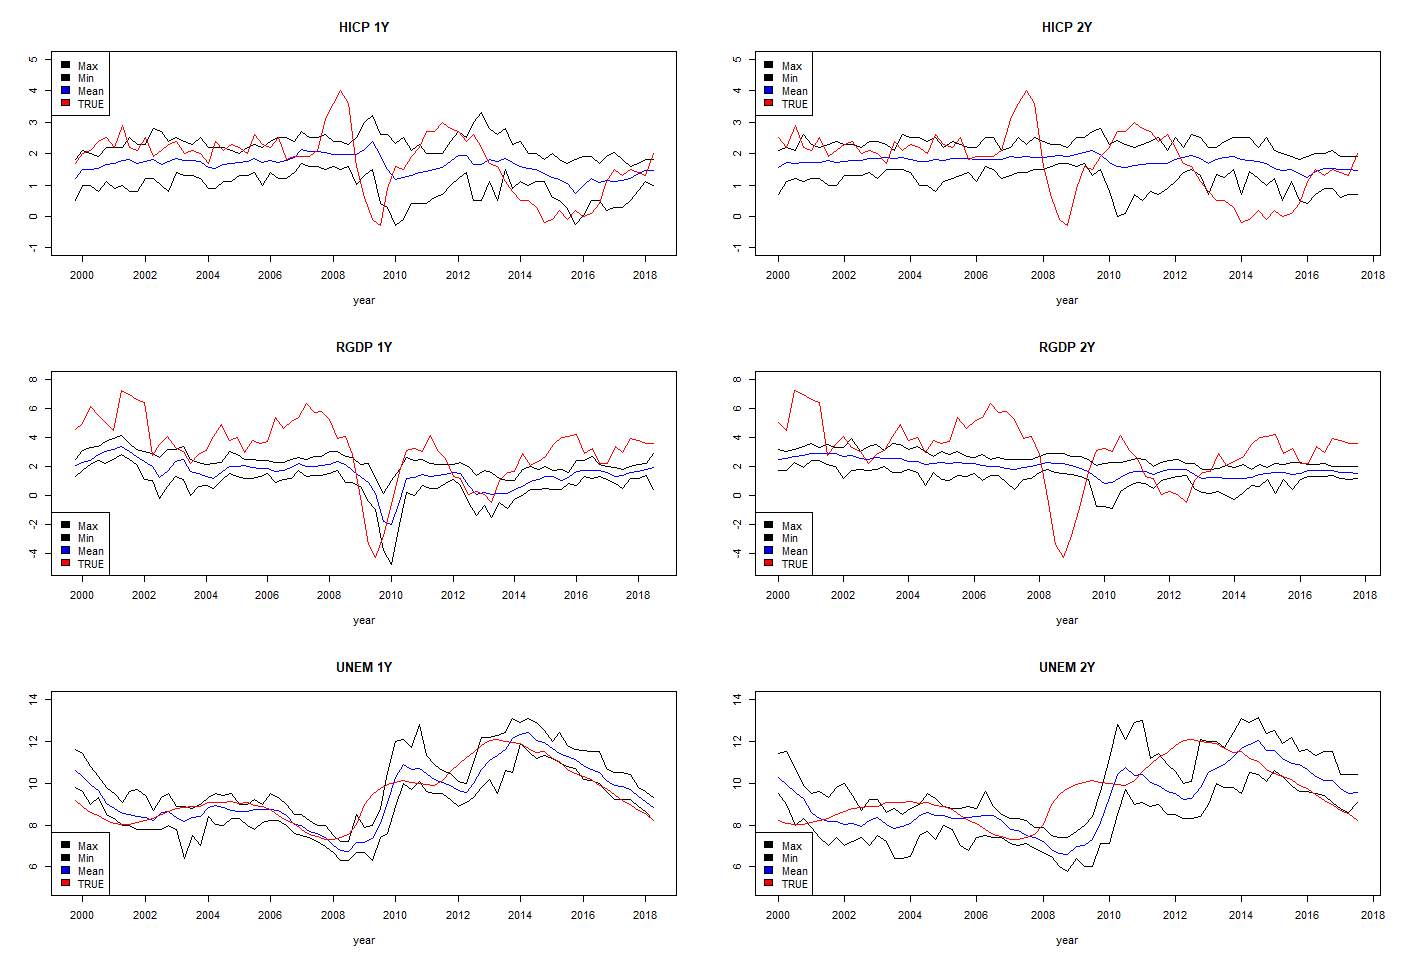
\includegraphics{./Images/SPF.pdf}
		\caption{Survey of Professional Forecasters data illustration}\label{fig: SPF data illustration}
	\end{figure}
	
	Figure \ref{fig: SPF data illustration} and Table \ref{tab: correlation summary statistics} show the plots of the forecasts alongside the true macroeconomic values and the statistics of the forecast errors' covariances, respectively. We plotted only the minimums, means, and maximums from the forecasts when constructing the plots in Figure 1. We see that there is high consistency across all forecasts, with the forecasts for two years ahead stronger than those for one year ahead. The consistency in the forecast is lower for the UNEM than for the other two. Furthermore, many true values lie outside of the forecast range, with the RGDP showing the worst results of the three in this regard. More values outside of the forecast range suggest that restricting the positive weight may be a strong limitation in the forecast combination.
	
	We examine the number of true values outside of the forecast range by looking at the summary statistics. Let the model space consist of an indicator with the value 1 when the true value is outside of the forecast range and 0 when the true value is inside. Table \ref{tab: modelspace summary statistics} shows the mean of the indicator. Of the three macro topics, the RGDP has the highest percentage of time periods outside of the forecast range, 83\%, followed by the HICP, with an average of 48\% of the time periods outside of the forecast range. The UNEM, at an average of 38\% of the time periods, has the lowest percentage of time periods outside the forecast range. Changing from one year out to two years out generally does not influence the mean of the indicator a great deal. Based on the results from Figure \ref{fig: SPF data illustration} and Table \ref{tab: modelspace summary statistics}, we expect that using truncation will have a large effect on the forecast of the RGDP, while it will not affect the forecasts of HICP and UNEM as much. We also expect that the two- years-ahead forecast will be better than the one-year-ahead forecast.
	
	\begin{table}[!h]
		\centering
		\caption{Means of the model space indicators for the forecasts for HICP, RGDP, and UNEM.}
		\label{tab: modelspace summary statistics}
		\begin{tabular}{lcccccc}
			\hline
			&\multicolumn{6}{c}{Model Space Indicator}\\
			\cmidrule(lr){2-7}
			Macro topic & \multicolumn{2}{c}{HICP} & \multicolumn{2}{c}{RGDP} & \multicolumn{2}{c}{UNEM} \\
			\cmidrule(lr){2-3} \cmidrule(lr){4-5}\cmidrule(lr){6-7}
			Horizon     & one year & two years & one year & two years & one year & two years \\ 
			\hline
			Mean        & 0.45        & 0.51         & 0.83        & 0.82        & 0.37         & 0.39       \\
			\hline
		\end{tabular}
	\end{table}
	
	As not all forecasters replied to each survey, we provide the number of forecasters per macroeconomic topic in Table \ref{tab: amount of forecasters}. The number of forecasters left after filtering is around 70 for one-year-ahead forecasts and 60 for two-years-ahead forecasts. We also show the number of replies per forecaster in a summary statistics table, Table \ref{tab: forecaster summary statistics}. The minimum number of forecasts is set to 24, and all forecasters with less than 24 forecasts are discarded. The maximum number of replies is around 70, which is close to the full 75 observations possible. With a mean of around 50, we have enough observations to compute pair-wise covariances, but the computation of a multivariate covariance is not fully supported.
	
	\begin{table}[!h]
		\centering
		\caption{Number of Forecasters.}
		\label{tab: amount of forecasters}
		\begin{tabular}{lcccccc}
			\hline
			&\multicolumn{6}{c}{Number of Forecasters}\\
			\cmidrule(lr){2-7}
			Macro topic & \multicolumn{2}{c}{HICP} & \multicolumn{2}{c}{RGDP} & \multicolumn{2}{c}{UNEM} \\
			\cmidrule(lr){2-3} \cmidrule(lr){4-5}\cmidrule(lr){6-7}
			Horizon     & one year & two years & one year & two years & one year & two years \\ 
			\hline
			Amount        &      72   &60          &70         &64         & 65         & 53       \\
			\hline
		\end{tabular}
	\end{table}
	
	\begin{table}[!h]
		\centering
		\caption{Summary statistics for the number of replies per forecaster per macro topic. Note: Means are rounded down to whole numbers for readability.}
		\label{tab: forecaster summary statistics}
		\begin{tabular}{lcccccc}%{S[table-format=3.2]}
			\hline
			&\multicolumn{6}{c}{Summary Statistics for the number of forecaster replies}\\
			\cmidrule(lr){2-7}
			Macro topic & \multicolumn{2}{c}{HICP} & \multicolumn{2}{c}{RGDP} & \multicolumn{2}{c}{UNEM} \\
			\cmidrule(lr){2-3} \cmidrule(lr){4-5}\cmidrule(lr){6-7}
			Horizon     & one year & two years & one year & two years & one year & two years \\ 
			\hline
			Minimum & 24    & 24    & 26    & 24    & 25    & 24    \\
			First Q & 40    & 40    & 42    & 35    & 40    & 36    \\
			Median  & 55    & 52    & 55    & 51    & 53    & 52    \\
			Mean    & 53    & 50    & 54    & 49    & 52    & 50    \\
			Third Q & 67    & 62    & 66    & 63    & 66    & 63    \\
			Maximum & 74    & 70    & 75    & 71    & 74    & 70      \\ 
			\hline
		\end{tabular}
	\end{table}
	
	Table \ref{tab: time summary statistics} shows the summary statistics for the number of survey replies per time period. On average there are 40 replies per time period. The deviation in the number of replies is small, with more than 50\% within the 35 to 45 range. The minimum of 22 for UNEM for two years ahead poses a possible problem in the estimation of the covariance. If the estimation of the covariance is poor, limiting negative weights will provide a better result.
	
	\begin{table}[!h]
		\centering
		\caption{Summary statistics for the survey reply numbers per time period.}
		\label{tab: time summary statistics}
		\begin{tabular}{lcccccc}%{S[table-format=3.2]}
			\hline
			&\multicolumn{6}{c}{Summary Statistics for the Number Per Time Period}\\
			\cmidrule(lr){2-7}
			Macro topic & \multicolumn{2}{c}{HICP} & \multicolumn{2}{c}{RGDP} & \multicolumn{2}{c}{UNEM} \\
			\cmidrule(lr){2-3} \cmidrule(lr){4-5}\cmidrule(lr){6-7}
			Horizon     & one year & two years & one year & two years & one year & two years \\ 
			\hline
			Minimum & 37    & 26    & 38    & 28    & 32    & 22    \\
			First Q & 43    & 35    & 42    & 36    & 38    & 30    \\
			Median  & 45    & 38    & 45    & 40    & 40    & 34    \\
			Mean    & 46    & 39    & 45    & 40    & 41    & 34    \\
			Third Q & 49    & 43    & 48    & 45    & 44    & 38    \\
			Maximum & 54    & 49    & 54    & 52    & 51    & 44       \\ 
			\hline
		\end{tabular}
	\end{table}
	
	Table \ref{tab: amount per test period} shows the number of replies per time period that we used to test the model. The values are lower than the mean for almost all of the time periods. Only the values for RGDP's one-year-ahead forecasts for 2018 Q1 and 2018 Q2 and UNEM's one-year-ahead forecast for 2016Q1 are above their averages. The low number above the mean decreases the dimension of the covariance matrix but, on the other hand, decreases the number of observations. Obtaining a lower dimension should be more important than the loss in observations.
	
	\begin{table}[!h]
		\centering
		\caption{Number of replies to the survey for the testing period starting in 2016. Note: All forecasters that replied during the test period had also replied in previous time periods.}
		\label{tab: amount per test period}
		\begin{tabular}{lcccccc}%{S[table-format=3.2]}
			\hline
			&\multicolumn{6}{c}{Survey Reply Numbers}\\
			\cmidrule(lr){2-7}
			Macro topic & \multicolumn{2}{c}{HICP} & \multicolumn{2}{c}{RGDP} & \multicolumn{2}{c}{UNEM} \\
			\cmidrule(lr){2-3} \cmidrule(lr){4-5}\cmidrule(lr){6-7}
			Test Period     & one year & two years & one year & two years & one year & two years \\ 
			\hline
			2016 Q1      & 45    & 32    & 38    & 33    & 41    & 30    \\
			2016 Q2      & 40    & 33    & 42    & 37    & 36    & 28    \\
			2016 Q3      & 44    & 35    & 42    & 38    & 39    & 28    \\
			2016 Q4      & 45    & 34    & 41    & 40    & 39    & 30    \\
			2017 Q1      & 39    & 35    & 38    & 30    & 32    & 32    \\
			2017 Q2      & 38    & 27    & 38    & 35    & 33    & 25    \\
			2017 Q3      & 37    & 31    & 43    & 36    & 33    & 29    \\
			2017 Q4      & 43    & 34    & 41    & 36    & 36    & 29    \\
			2018 Q1      & 40    & 27    & 46    & 30    & 34    & 22    \\
			2018 Q2      & 44    & 26    & 45    & 31    & 40    & 23    \\ 
			\hline
		\end{tabular}
	\end{table}
	
	Table \ref{tab: correlation summary statistics} provides  information on how the forecast errors are correlated. The diagonal elements of the correlation matrix are not reported in the table. For all of the series, the correlations are, on average, above 60\%. For HICP and UNEM, the correlation increases across all statistics when the forecast horizon increases, while, for RGDP, it remains the same. The lowest correlation to be found is -0.02 for UNEM, but this number is not too different from the minimum correlations for the other two topics.
	
	\begin{table}[!h]
		\centering
		\caption{Summary statistics of the correlations of the forecast errors.}
		\label{tab: correlation summary statistics}
		\begin{tabular}{lcccccc}%{S[table-format=3.2]}
			\hline
			&\multicolumn{6}{c}{Correlation}\\
			\cmidrule(lr){2-7}
			Macro topic & \multicolumn{2}{c}{HICP} & \multicolumn{2}{c}{RGDP} & \multicolumn{2}{c}{UNEM} \\
			\cmidrule(lr){2-3} \cmidrule(lr){4-5}\cmidrule(lr){6-7}
			Horizon     & one year & two years & one year & two years & one year & two years \\ 
			\hline
			Minimum     & 0.03        & 0.02        & 0.11        & 0.13        & -0.02        & 0.08       \\
			First Q     & 0.53        & 0.62        & 0.63        & 0.65        & 0.47         & 0.56       \\
			Mean        & 0.64        & 0.70        & 0.75        & 0.75        & 0.59         & 0.67       \\
			Median      & 0.66        & 0.72        & 0.81        & 0.80        & 0.62         & 0.70       \\
			Third Q     & 0.77        & 0.81        & 0.89        & 0.87        & 0.74         & 0.80       \\
			Maximum     & 0.96        & 0.97        & 0.98        & 0.98        & 0.94         & 0.95       \\ 
			\hline
		\end{tabular}
	\end{table}
	
	
	We conclude that the SPF exhibits characteristics that are not in the standard assumption where the correlations are close to 0. By incorporating the possibility of negative weights, we expect to see some improvement in the forecast errors.
	
	\section{Empirical Results}\label{empirical-results}
	\subsection{Optimal Weight}\label{optimal-weight}
	An analysis of the optimal weight given by Equation \ref{eqn: simple weight} provides us with a preliminary understanding of the variability. Table \ref{tab: simple weight summary statistics} shows the summary statistics for the optimal weight. We see that for all macroeconomic topics, the mean and median vary around 0.02, which is close to the calculation obtained when using equal weights. Looking at the first and the third quantile, we see that half of the weights are between -0.6 and 0.6, which gives us a possible range of effectiveness for the threshold. The minimums and maximums are extreme considering that 1 is 100\%. With values as low at -11, -14, and -21 for HCIP, RGDP, and UNEM, respectively, and the first and third quartiles only down to -0.6 and up to 0.6 at most, the distribution of the weights indicates a strong thick-tail behaviour. When considering the difference between one year and two years ahead, for two out of three macro topics, the extreme values converge to 0. RGDP becomes more volatile when the horizon increase from one to two years. On the other hand, the gap between the first and third quantile increases for all topics between one year and two years ahead. This increase indicates an increase in the choices of negative weights for the two-year horizon. The means and medians do not change much in relation to the forecast horizon.
	
	\begin{table}[!h]
		\centering
		\caption{Summary statistics for the weight from Equation \ref{eqn: simple weight}.}
		\label{tab: simple weight summary statistics}
		\begin{tabular}{lcccccc}%{S[table-format=3.2]}
			\hline
			&\multicolumn{5}{c}{Optimal Weight}\\
			\cmidrule(lr){2-7}
			Macro topic & \multicolumn{2}{c}{HICP} & \multicolumn{2}{c}{RGDP} & \multicolumn{2}{c}{UNEM} \\
			\cmidrule(lr){2-3} \cmidrule(lr){4-5}\cmidrule(lr){6-7}
			Horizon     & one year & two years & one year & two years & one year & two years \\ 
			\hline
			Minimum      & -11.05      & -6.21      & -9.00      & -21.79      & -14.41      & -5.64      \\
			First Q      & -0.30       & -0.59      & -0.20      & -0.63       & -0.28       & -0.40      \\
			Mean         & 0.04        & 0.04       & 0.01       & -0.01       & 0.03        & 0.05       \\
			Median       & 0.05        & 0.03       & 0.04       & 0.01        & 0.04        & 0.03       \\
			Third Q      & 0.41        & 0.60       & 0.25       & 0.82        & 0.39        & 0.43       \\
			Maximum      & 12.94       & 7.56       & 8.74       & 16.34       & 11.26       & 7.90       \\ 
			\hline
		\end{tabular}
	\end{table}
	
	\subsection{Procedure}\label{procedure}
	
	We seek to evaluate the effect of truncating the weight when using the SPF data. The procedure for obtaining the weight can differ between researchers. Therefore, we provide the exact steps taken in the weight estimation below:
	
	
	Given each time to forecast, we use all of the known observations before that forecast time period.
	
	\begin{enumerate}
		\def\labelenumi{\arabic{enumi}.}
		\item
		Find the nearest positive definite covariance matrix. This step is required for the covariance to be invertible. We employ the nearPD function from the R package \emph{Matrix}. The nearPD function first decomposes the covariance into a univariate variance and the correlation. The function then uses the algorithm \emph{higham} on the correlation matrix to compute the nearest positive definite matrix. The final result is a covariance matrix that is a combination of the univariate variance and the correlation matrix.
		\item
		Subset of the covariance. We find the submatrix containing only the available forecasts for the testing period. If 80 forecasters had made previous forecasts, but only 40 of them made forecasts for the testing period, we discard the 40 extra forecasters.
		\item
		Estimate the optimal weight \(w^*\) using Equation
		\ref{eqn: simple weight}.
		\item
		Truncate the optimal weight with Equation \ref{eqn: w trunc}. The weight now has fewer values, which do not sum to one. We normalise the weights back such that the sum of the weights is 1.
		\item
		Combine the forecast using the new weights.
		\item
		Calculate the test statistics for the new weights and equal weights.
		\item
		Calculate the ratio of the test statistics for the new weights to the equal weights.
	\end{enumerate}
	
	\subsection{Ratio of Test Statistics}\label{ratio-of-test-statistics}
	The ratio of test statistics is determined by evaluating the performance of the various weights using the mean absolute prediction error (MAPE) and mean squared prediction error (MSPE). A comparison is then made between the MSPE of equal weights and the truncated MAPE and MSPE, respectively, for the same weight by creating the test ratios. The results for the UNEM, RGDP and HICP are then documented, and the ratios involving the MAPE and MSPE are reported to assist in the visualisation of the impact of truncation. The statistics for the truncation is considered to be smaller than the statistic for the same weight if its value is less than 1. The weights below the threshold $c$ are set to $c$.
	
	In Table \ref{tab: c MSPE HICP},  using various truncation values, the ratios are obtained for one-year and two-year horizons. The minimum MAPE ratio is attained at -1 and -1.5 for the one-year and two-year horizons, respectively. The two-year choice or selection of threshold based on the MAPE ratio is the same as that made based on the MSPE, i.e., -1.5. Furthermore, -1.5 is the only threshold with a MAPE ratio lower than 1 for the two-year horizon. The MSPE ratio is farthest below 1 at 0.91 (threshold of -0.5) and 0.93 (threshold of -1.5) for the 1- and 2-year horizons. This effect is not strongly visible for the MAPE ratio.
	
	\begin{table}[!h]
		\centering
		\caption{Mean Squared Prediction Error (MSPE) and Mean Absolute Prediction Error (MAPE) ratios for inflation with different truncation values for the weight.}
		\label{tab: c MSPE HICP}
		\begin{tabular}{lcccc}
			\hline\hline
			&                        \multicolumn{4}{c}{HICP}                         \\
			\cmidrule(lr){2-5}                              & \multicolumn{2}{c}{One-Year Horizon} & \multicolumn{2}{c}{Two-Year Horizon} \\
			\cmidrule(lr){2-3} \cmidrule(lr){4-5}
			Threshold & MSPE Ratio &    MAPE Ratio    & MSPE Ratio &    MAPE Ratio    \\ \hline
			-$\infty$ & 3.2902 & 1.5898 & 2.2072 & 1.4347\\ 
			-5 & 2.8209 & 1.4174 & 2.0871 & 1.3563\\ 
			-4.5 & 2.8209 & 1.4175 & 2.0296 & 1.2925\\ 
			-4 & 2.8208 & 1.4173 & 2.0475 & 1.3145\\ 
			-3.5 & 2.8203 & 1.4166 & 1.8539 & 1.268\\ 
			-3 & 2.8196 & 1.4156 & 1.6821 & 1.212\\ 
			-2.5 & 2.8191 & 1.4147 & 1.2439 & 1.1119\\ 
			-2 & 2.0779 & 1.2606 & 1.0318 & 1.0604\\ 
			-1.5 & 1.1934 & 1.0686 & 0.925 & 0.9852\\ 
			-1 & 0.9389 & 0.9819 & 0.9587 & 1.029\\ 
			-0.5 & 0.9101 & 0.9875 & 0.9724 & 1.0201\\ 
			0 & 0.9844 & 0.9994 & 0.9834 & 1.0005\\ 
			\hline\hline
		\end{tabular}
	\end{table}
	
	Table \ref{tab: c MSPE RGDP} reports the same information for the RGDP.  The one-year thresholds are at approximately -1 and -1.5 for the MSPE (0.83) and MAPE (0.89) ratios, respectively. For the two-year horizon, the MAPE ratio behaves differently, reaching its lowest value below 1 at a threshold of -5. However, the MSPE ratio did not go below 1 in the threshold range between -5 and 0. We did not search below -5 for the threshold. The boundary that is realized due to this cut-off occurs at1.01 at a threshold of 0. The smallest MAPE ratio for the two-year horizon (0.91) occurs at a threshold of -4.5. When considering the one-year horizon, the optimal weight MSPE ratio has a score of 1.44, showing that it is similar to what occurs at equal weights. With a ratio of 6.07, on the other hand, the two-year horizon does not seem to perform so well at optimal weight. For the one- and two-year horizons, the optimal MAPE ratios (1.80 and 1.07, respectively)  are similar to what would occur under equal weights.
	
	\begin{table}[!h]
		\centering
		\caption{Mean Squared Prediction Error (MSPE) and Mean Absolute Prediction Error (MAPE) ratios for economic growth at various truncation values for the weights.}
		\label{tab: c MSPE RGDP}
		\begin{tabular}{lcccc}
			\hline\hline
			&                        \multicolumn{4}{c}{RGDP}                         \\
			\cmidrule(lr){2-5}                              & \multicolumn{2}{c}{One-Year Horizon} & \multicolumn{2}{c}{Two-Year Horizon} \\
			\cmidrule(lr){2-3} \cmidrule(lr){4-5}
			Threshold & MSPE Ratio &    MAPE Ratio    & MSPE Ratio &    MAPE Ratio    \\ \hline
			-$\infty$ & 1.4387 & 1.0681 & 6.0654 & 1.8047\\ 
			-5 & 1.0854 & 0.944 & 1.0474 & 0.9234\\ 
			-4.5 & 1.0911 & 0.9491 & 1.0385 & 0.9087\\ 
			-4 & 1.1081 & 0.9622 & 1.0445 & 0.9277\\ 
			-3.5 & 1.1021 & 0.9657 & 1.0537 & 0.9401\\ 
			-3 & 0.9826 & 0.9389 & 1.0571 & 0.9462\\ 
			-2.5 & 0.9076 & 0.9164 & 1.0663 & 0.9604\\ 
			-2 & 0.8654 & 0.8987 & 1.0722 & 0.9677\\ 
			-1.5 & 0.8408 & 0.8856 & 1.0847 & 0.977\\ 
			-1 & 0.8309 & 0.8894 & 1.1191 & 1.0273\\ 
			-0.5 & 0.8523 & 0.9125 & 1.047 & 1.0219\\ 
			0 & 0.9721 & 0.9844 & 1.0073 & 1.0056\\ 
			\hline\hline
		\end{tabular}
	\end{table}
	
	If we take a close look at the UNEM, the results tend to give ratios that are promising. The lowest MSPE ratios for the one-year and two-year horizons were registered at -1 and 0, respectively. As stated previously, we did not search below a threshold of -5 in this thesis. Compared to the MSPE ratios obtained for HICP and RGDP, the MSPE ratios of 0.60 and 0.83 obtained for UNEM for the one- and two-year horizons, respectively, are the lowest of the three.  Moreover, the lowest MAPE one-year ratio of 0.73 and the two-year ratio of 0.90 at -1.5 and -0.5, respectively, provide positive news. It is interesting that the optimal weight for the one-year MAPE ratio is already 0.89. This is lower than it was for the other macroeconomic topics.
	
	\begin{table}[!h]
		\centering
		\caption{Mean Squared Prediction Error (MSPE) and Mean Absolute Prediction Error (MAPE) ratios for unemployment at various truncation values for the weights.}
		\label{tab: c MSPE UNEM}
		\begin{tabular}{lcccc}
			\hline\hline
			&                        \multicolumn{4}{c}{UNEM}                         \\
			\cmidrule(lr){2-5}                              & \multicolumn{2}{c}{One-Year Horizon} & \multicolumn{2}{c}{Two-Year Horizon} \\
			\cmidrule(lr){2-3} \cmidrule(lr){4-5}
			Threshold & MSPE Ratio &    MAPE Ratio    & MSPE Ratio &    MAPE Ratio    \\ \hline
			-$\infty$ & 1.1639 & 0.8899 & 4.3535 & 1.6517\\ 
			-5 & 1.0247 & 0.8437 & 3.1368 & 1.5265\\ 
			-4.5 & 0.863 & 0.7843 & 2.8128 & 1.481\\ 
			-4 & 0.8159 & 0.7345 & 2.5409 & 1.4332\\ 
			-3.5 & 0.8384 & 0.7679 & 2.3461 & 1.3901\\ 
			-3 & 0.8718 & 0.7893 & 2.1681 & 1.332\\ 
			-2.5 & 0.8885 & 0.7972 & 2.0443 & 1.2694\\ 
			-2 & 0.8206 & 0.7977 & 1.9581 & 1.2442\\ 
			-1.5 & 0.6761 & 0.7379 & 1.8529 & 1.2262\\ 
			-1 & 0.6033 & 0.6819 & 1.55 & 1.0992\\ 
			-0.5 & 0.6454 & 0.725 & 1.0037 & 0.933\\ 
			0 & 0.9346 & 0.9543 & 0.8769 & 0.9466\\ 
			\hline\hline
		\end{tabular}
	\end{table}
	
	Based on Figure \ref{fig: c Ratio sub}, with plots created using a 0.1 step size, HICP inhibits a relatively quick reduction in both minor changes and statistics. RGDP shows an increase in the lower threshold for a one-year horizon and a U-shape thereafter. RGDP with a two-year horizon exhibits odd behaviour by showing first a U-shape around a threshold of -4.5 and then a drop after -1. UNEM with a one-year horizon exhibits a W-shaped error, indicating that the changes in variance reduction and/or bias increments are not gradual. UNEM for a two-year horizon, on the other hand, has a consistently downward slope as the threshold is increased.
	
	\begin{figure}[!h]
		\centering
		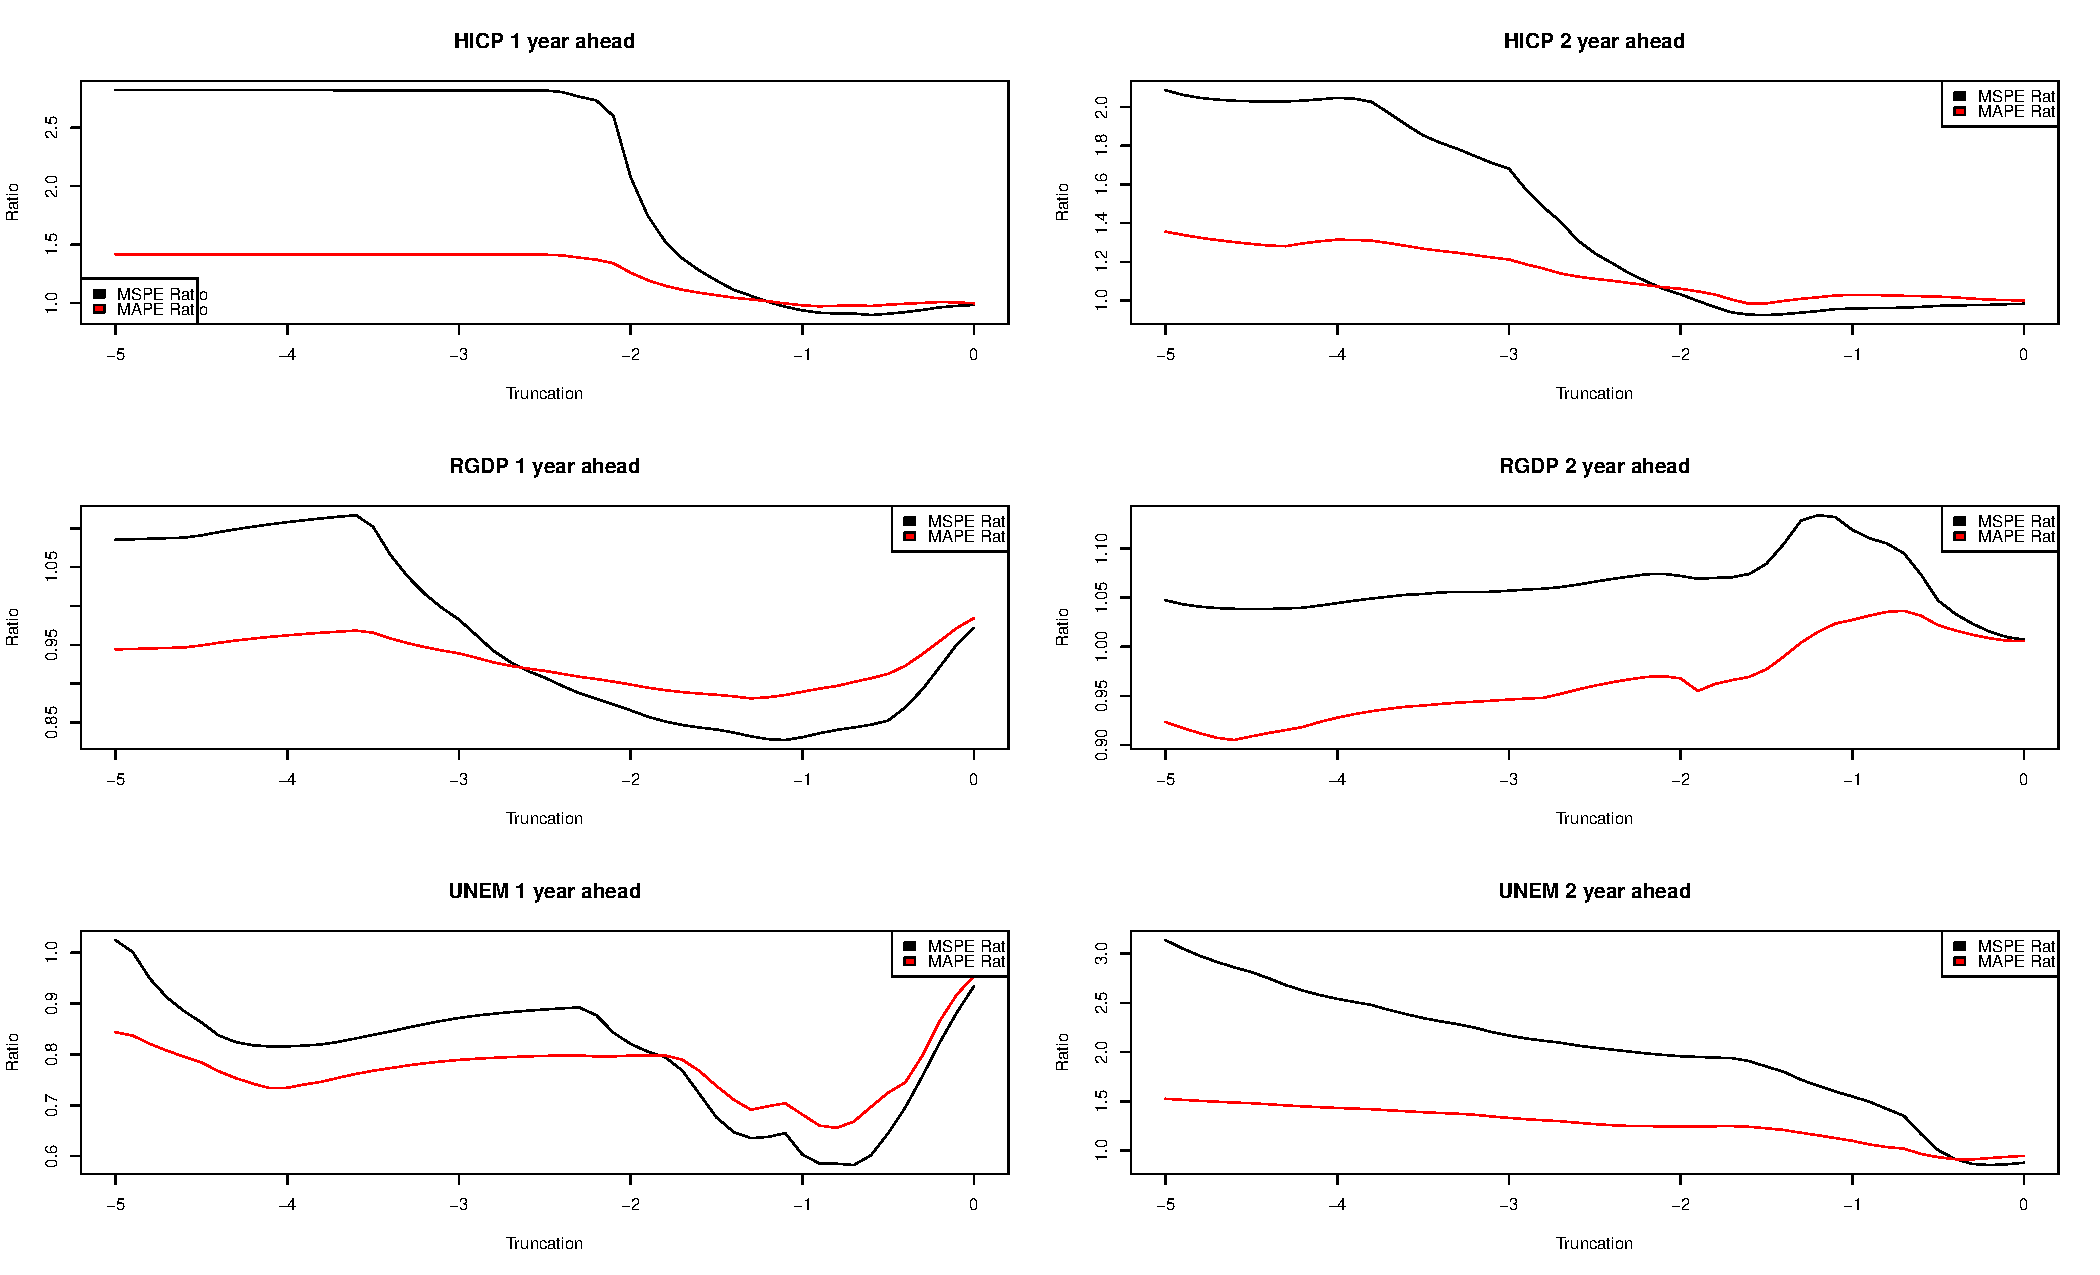
\includegraphics{./Images/Ratio_c.pdf}
		\caption{MSPE ratios for the different macroeconomic topics}\label{fig: c Ratio sub}
	\end{figure}
	
	This section shows that it is possible to outperform equal weights and no negative weights under certain circumstances. Five out of six macroeconomic scenarios show positive news. The results are promising, as we have shown that there is no need to go fully in removing the covariance.
	
	\subsection{Ratio with $c$ as $0$}\label{ratio-of-mean-squared-prediction-error}
	Section \ref{ratio-of-test-statistics} illustrates the effects of truncation. This section considers a special truncation case. Any weights that are below the threshold are set to $0$. In other words, doing so effectively removes the forecasts associated with those weights. This is an interesting case due to the intersection between the threshold and variable selection. The differences found between Section \ref{ratio-of-test-statistics} and Section \ref{ratio-of-mean-squared-prediction-error} can then be explained partially by the differences in forecast combination and forecast selection.
	
	We see in Table \ref{tab: MSPE HICP} that for the truncation values -2 and -1.5, the minimum MSPE ratios for HICP are attained for the one- and two-year horizons, respectively. The minimum MAPE ratios are obtained for the one-and two-year horizons at -2 and 0, respectively. The one-year selection of the threshold based on the MAPE ratio coincides with selection based on the MSPE ratio, but the minimum for the MAPE ratio is not at a threshold of -1.5 for a two-year horizon. The optimal weight provides MSPE ratios of 3.29 and 2.21 for the one- and two-year horizons, respectively, but the ratios are significantly larger than the ratios obtained via truncation. The differences in the MAPE ratios between  the optimal and truncated weights are smaller compared to what occurs with the MSPE ratio. Truncating all the way to 0 means that no forecast with a weight less than 0 is used in the final forecast. For HICP, selecting too strict a threshold does not help in 3 out of 4 cases.
	
	
	\begin{table}[!h]
		\centering
		\caption{Mean Squared Prediction Error (MSPE) and Mean Absolute Prediction Error (MAPE) ratios for inflation with the truncation value set to 0.}
		\label{tab: MSPE HICP}
		\begin{tabular}{lcccc}
			\hline\hline
			&                        \multicolumn{4}{c}{HICP}                         \\
			\cmidrule(lr){2-5}                              & \multicolumn{2}{c}{One-Year Horizon} & \multicolumn{2}{c}{Two-Year Horizon} \\
			\cmidrule(lr){2-3} \cmidrule(lr){4-5}
			Threshold & MSPE Ratio &    MAPE Ratio    & MSPE Ratio &    MAPE Ratio    \\ \hline
			-$\infty$ & 3.2902 & 1.5898 & 2.2072 & 1.4347\\ 
			-5 & 2.8211 & 1.4178 & 2.1148 & 1.3537\\ 
			-4.5 & 2.8211 & 1.4178 & 2.1148 & 1.3537\\ 
			-4 & 2.8187 & 1.414 & 2.1500 & 1.3753\\ 
			-3.5 & 2.8178 & 1.4126 & 1.6747 & 1.1988\\ 
			-3 & 2.8178 & 1.4126 & 1.5479 & 1.1551\\ 
			-2.5 & 2.8180 & 1.4129 & 1.0181 & 1.0638\\ 
			-2 & 0.8078 & 0.9025 & 0.993 & 1.0653\\ 
			-1.5 & 0.8877 & 0.9619 & 0.9688 & 1.0390\\ 
			-1 & 0.8835 & 0.9610 & 0.9764 & 1.0170\\ 
			-0.5 & 0.9465 & 0.9912 & 0.9877 & 1.0108\\ 
			0 & 0.9844 & 0.9994 & 0.9834 & 1.0005\\ 		 \hline\hline
		\end{tabular}
	\end{table}
	
	Table \ref{tab: MSPE RGDP} shows a similar pattern for RGDP. The optimal threshold for the one-year horizon is around -1.5, where the values of the MSPE and MAPE ratios are 0.83 and 0.88, respectively. We did not look for a threshold larger than 0, and the minimum MSPE ratio for a two- year horizon was not within the search region. This cut-off gives us 1.01 as the boundary case. The MAPE ration for the two-year horizon behaves differently. The minimum MAPE ratio is achieved at -4.5. The optimal-weight MSPE ratio (1.44) for the one-year horizon is similar to that for equal weights. The two-year horizon MSPE ratio, on the other hand, does not perform that well at optimal weight since it has a value of 6.07. The optimal-weight MAPE ratios for the one- and two-year horizons have values similar to those for equal weights at 1.07 and 1.80, respectively.
	
	\begin{table}[!h]
		\centering
		\caption{Mean Squared Prediction Error (MSPE) and Mean Absolute Prediction Error (MAPE) ratios for economic growth with the truncation value set to 0.}
		\label{tab: MSPE RGDP}
		\begin{tabular}{lcccc}
			\hline\hline
			& \multicolumn{4}{c}{RGDP}                                                \\
			\cmidrule(lr){2-5}
			& \multicolumn{2}{c}{One-Year Horizon} & \multicolumn{2}{c}{Two-Year Horizon} \\
			\cmidrule(lr){2-3} \cmidrule(lr){4-5}
			Threshold & MSPE Ratio &    MAPE Ratio    & MSPE Ratio &    MAPE Ratio    \\ 
			\hline
			-$\infty$ & 1.4387 & 1.0681 & 6.0654 & 1.8047\\ 
			-5 & 1.1000 & 0.9561 & 1.0684 & 0.9496\\ 
			-4.5 & 1.1462 & 0.9861 & 1.0683 & 0.9496\\ 
			-4 & 1.1462 & 0.9861 & 1.0885 & 0.9621\\ 
			-3.5 & 0.8738 & 0.9029 & 1.0765 & 0.9539\\ 
			-3 & 0.8768 & 0.9046 & 1.0824 & 0.9579\\ 
			-2.5 & 0.8611 & 0.8967 & 1.102 & 0.9899\\ 
			-2 & 0.8402 & 0.8824 & 1.0824 & 0.9567\\ 
			-1.5 & 0.8278 & 0.8768 & 1.1712 & 1.0438\\ 
			-1 & 0.8610 & 0.9102 & 1.1356 & 1.0617\\ 
			-0.5 & 0.8999 & 0.9396 & 1.0198 & 1.0114\\ 
			0 & 0.9721 & 0.9844 & 1.0073 & 1.0056\\  \hline\hline
		\end{tabular}
	\end{table}
	
	
	When we look further into the UNEM, the results show well-performing ratios. UNEM achieved the lowest MSPE ratios for the one- and two-year horizons at thresholds of -1.5 and -0.5, respectively. Compared to HICP and RGDP, the MSPE ratios of 0.70 and 0.82 for the one- and two-year horizons, respectively, are the lowest of the three. The MSPE ratio of 0.70 also shows a 40\% decrease in the MSPE, even when the non-truncated value was already at 1.16. The MAPE ratio shows that when looking at the one-year horizon, the optimal weight already outperforms equal weights with a ratio of 0.89, but, with truncation, the MAPE ratio drops further to 0.74. The MAPE ratio for the two-year horizon decreases to 0.91. UNEM seems to have been affected by the truncation in a manner that is not explained by the correlations. UNEM does not have a difference in correlations compared to the other macroeconomics topics that cannot be explained by estimation noise. One possible explanation for what is happening is that the optimal choice for the truncation is more consistent over time. We will evaluate the consistency of the truncation in the out-of-sample (OOS) selection area.
	
	\begin{table}[!h] 
		\centering
		\caption{Mean Squared Prediction Error (MSPE) and Mean Absolute Prediction Error (MAPE) ratios for unemployment with the truncation value set to 0.}
		\label{tab: MSPE UNEM}
		\begin{tabular}{lcccc}
			\hline\hline
			& \multicolumn{4}{c}{UNEM}                                                \\
			\cmidrule(lr){2-5}
			& \multicolumn{2}{c}{One-Year Horizon} & \multicolumn{2}{c}{Two-Year Horizon} \\
			\cmidrule(lr){2-3} \cmidrule(lr){4-5}
			Threshold & MSPE Ratio &    MAPE Ratio    & MSPE Ratio &    MAPE Ratio    \\ 
			\hline
			-$\infty$ & 1.1639 & 0.8899 & 4.3535 & 1.6517\\ 
			-5 & 1.0249 & 0.8438 & 2.3189 & 1.3796\\ 
			-4.5 & 0.8926 & 0.7991 & 2.3189 & 1.3796\\ 
			-4 & 0.8926 & 0.7991 & 2.2467 & 1.3552\\ 
			-3.5 & 0.9447 & 0.8189 & 2.0462 & 1.3042\\ 
			-3 & 0.9335 & 0.8137 & 1.9501 & 1.2435\\ 
			-2.5 & 0.9097 & 0.8050 & 1.9146 & 1.2427\\ 
			-2 & 0.7684 & 0.7858 & 1.8718 & 1.2264\\ 
			-1.5 & 0.6988 & 0.7399 & 1.6610 & 1.1328\\ 
			-1 & 0.7283 & 0.7554 & 1.4222 & 1.0346\\ 
			-0.5 & 0.8232 & 0.8471 & 0.8242 & 0.9066\\ 
			0 & 0.9346 & 0.9543 & 0.8769 & 0.9466\\ \hline\hline
		\end{tabular}
	\end{table}
	
	
	Figure \ref{fig: Ratio sub} shows the MSPE ratios and MAPE ratios for HICP, RGDP, and UNEM with forecast horizons of one and two years. The figures are plotted with a step size of 0.1. From the figure, it can be seen that HICP shows a sudden decrease in both statistics and minor changes. RGDP with a one-year horizon shows a similar pattern with a larger increase towards the end. For RGDP with a two-year horizon, there is a spike in both statistics around a threshold of 1.3. Given that the value never falls below 1, we suspect that the correlation does not capture the error well enough, and there might be a better measure that can be used to counter the forecast error. UNEM with a one-year horizon is a bit volatile but exhibits a well-defined U-shape. For UNEM with a two-year horizon, the ratios decrease smoothly to the minimum.
	
	\begin{figure}[!h]
		\centering
		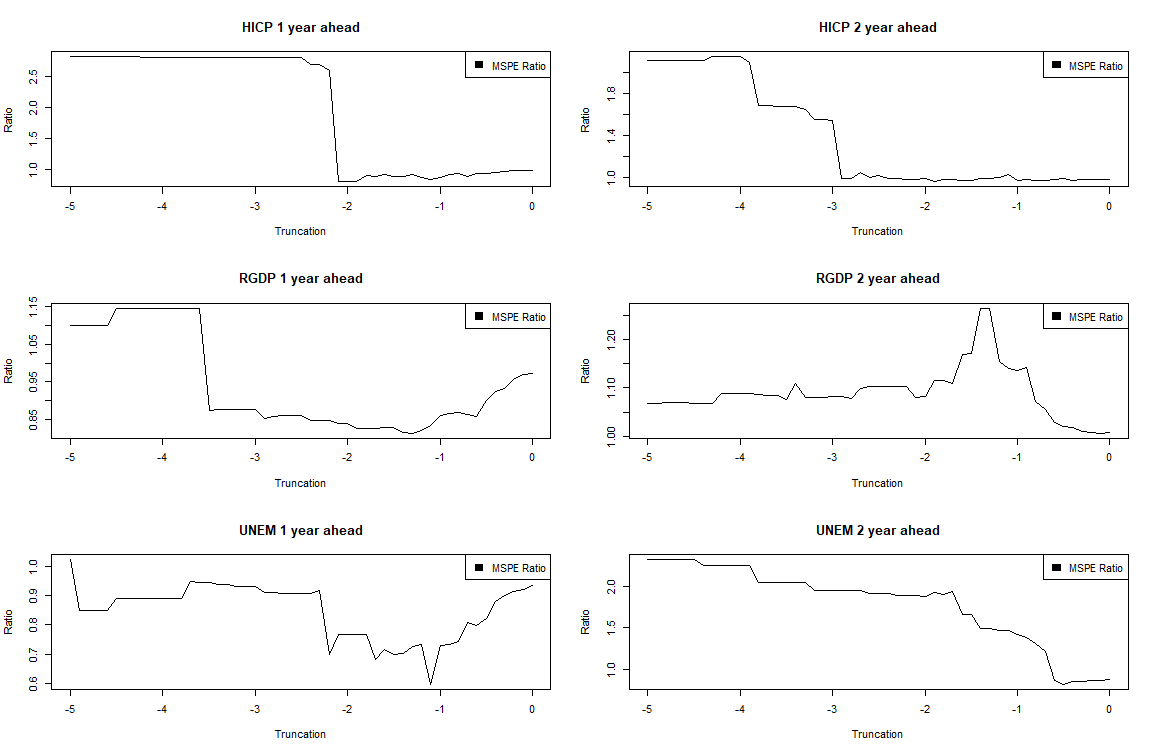
\includegraphics{./Images/Ratio.pdf}
		\caption{MSPE ratios for the different macroeconomic topics}\label{fig: Ratio sub}
	\end{figure}
	
	To conclude, we see the possibility of improving the MSPE and MAPE ratios with truncation in all cases. In the beginning, there is a drop in the test statistics, but, closer to the threshold of 0, the test statistics increase. The MSPE and MAPE ratios both have U-shaped characteristics, attributed to the variances and biases. When truncation is applied, the drop in the variance is larger than the increase in the bias, contributing to the decrease in the test statistics. It is worth noting that all of the macroeconomic topics have exhibited, on average, better performances than possible when using equal weights, which is considered a benchmark that is hard to beat. Two of the macroeconomic two-year forecasts (for HICP and RGDP) have a hard time justifying the improvement in the MSPE or MAPE ratio when the estimation errors are taken into consideration. The remaining four forecasts achieve between 17\% and 30\% decreases when compared to what would have been possible using equal weights. The results also show that the decrease in the MSPE is not just for one point, but rather a gradual movement. Even if the user does not select the most optimal case, but deviates from it by a small amount, the increase in the test statistics is relatively contained. Hence, the truncation selection process is robust.
	
	\subsection{Optimal Truncation Selection}\label{out-of-sample-truncation-selection}
	
	In this section, we examine the MSPE and MAPE ratios with regards to weight truncation when the truncation parameter is in-sample optimally selected. To make the selection of the truncation parameter, we follow the following steps:
	
	\begin{enumerate}
		\def\labelenumi{\arabic{enumi}.}
		\item
		Estimate the optimal weight in Equation \ref{eqn: simple weight}.
		\item
		Calculate the in-sample mean squared error (MSE) with the truncated weight, e.g., the first window is 1999 Q4 to 2015 Q4. The truncation parameter ranges from -10 to 0 with a step of 0.1. We also look into other starting values, namely, -5, -2, and -1.
		\item
		Select the truncation parameter with the lowest in-sample MSE.
		\item
		Use the selected truncation parameter to combine the predictions.
		\item
		Calculate the test statistics of the new weights and equal weights.
		\item
		Calculate the ratio of the test statistics of new weights to the equal weights.
	\end{enumerate}
	
	If there are multiple truncation points with the same MSE value, we will take the largest truncation value of those having the same MSE. The reason for choosing the largest value is that the threshold is then closer to the next changing point in the MSE. Assume, for example, that a weight with a minimum of -1 is optimal and that any higher weight results in a higher MSE value. Further, suppose that all truncation values between -10 and -1 result in the same minimal MSE. We would therefore choose -1 to record. The choice does not influence the forecast and is chosen purely for the analysis to take place later.
	
	\subsection{Optimal Truncation Selection Results}\label{out-of-sample-truncation-result}
	We evaluate the Optimal Truncation (OT) forecasting ability using the methods in Section \ref{ratio-of-mean-squared-prediction-error}. The MSPE and MAPE ratios are given in Table \ref{tab: oos mspe}.
	
	As shown in Table \ref{tab: oos mspe}, OT improves all MSPE values when we compare them with the values obtained for equal weights. When considering the MAPE ratios, OT failed to improve the HICP one-year horizon, but obtained it produced positive results for the other five scenarios. The truncation works better for RGDP and UNEM. If we compare the values of the MSPE or MAPE ratios for the optimal weights, we see that the truncation improves the forecasts for all topics except UNEM with a one-year horizon. RGDP with a two-year horizon also shows via the MSPE ratios that none of the constant truncations works as well as a changing truncation. This means that the optimal truncation selection overweighs the selection uncertainty. These results verify the idea that the truncation improves upon equal weights even if the truncation uncertainty can increase the MSPE. 
	
	Table \ref{tab: oos mspe} also illustrates the effect of changing the search area. A smaller search area results in less uncertainty but is more restrictive in terms of the solution space. In the cases of the HICP one-year horizon and the  UNEM two-year horizon, changing the search area does not influence the test statistics enough to be visible to four places. For the HICP two-year horizon and the RGDP one-year horizon, being more restrictive increases the test statistics, effectively resulting in poorer predictions. For the RGDP two-year horizon and the UNEM one-year horizon, being restrictive decreases the prediction errors and therefore the MSPE and MAPE ratios. Since choosing to be restrictive or not depends on prior information on the forecast set, it is hard to determine what a good choice is.
	
	\begin{table}[!h]
		\centering
		\caption{Mean Squared Prediction Error ratio and Mean Absolute Prediction Error ratio when the selection of the truncation is optimal. The minimum search to optimal thresholds are -10, -5, -2, and -1.}
		\label{tab: oos mspe}
		\begin{tabular}{lcccccc}
			\hline
			&\multicolumn{6}{c}{MSPE with Optimal Truncation}\\
			\cmidrule(lr){2-7}
			Macro topic & \multicolumn{2}{c}{HICP} & \multicolumn{2}{c}{RGDP} & \multicolumn{2}{c}{UNEM} \\
			\cmidrule(lr){2-3} \cmidrule(lr){4-5}\cmidrule(lr){6-7}
			Threshold     & one year & two years & one year & two years & one year & two years \\ 
			\hline
			-10 & 0.9670   & 0.9611   & 0.9275   & 0.9558   & 0.9153   & 0.8752   \\ 
			-5  & 0.9670   & 0.9611   & 0.9275   & 0.9558   & 0.9153   & 0.8752   \\ 
			-2  & 0.9670   & 0.9719   & 0.9319   & 0.9518   & 0.8982   & 0.8752   \\ 
			-1  & 0.9670   & 0.9709   & 0.9319   & 0.9949   & 0.8982   & 0.8752   \\ 
			\hline
			&\multicolumn{6}{c}{MAPE with Optimal Truncation}\\
			\cmidrule(lr){2-7}
			Macro topic & \multicolumn{2}{c}{HICP} & \multicolumn{2}{c}{RGDP} & \multicolumn{2}{c}{UNEM} \\
			\cmidrule(lr){2-3} \cmidrule(lr){4-5}\cmidrule(lr){6-7}
			Threshold     & one year & two years & one year & two years & one year & two years \\ 
			\hline
			-10 & 1.0015   & 0.9928   & 0.9532   & 0.9577   & 0.9320   & 0.9502   \\
			-5  & 1.0015   & 0.9928   & 0.9532   & 0.9577   & 0.9320   & 0.9502   \\
			-2  & 1.0015   & 0.9968   & 0.9562   & 0.9533   & 0.9260   & 0.9502   \\
			-1  & 1.0015   & 0.9988   & 0.9562   & 0.9524   & 0.9260   & 0.9502   \\
			\hline
		\end{tabular}
	\end{table}
	
	To better understand the OT, Table \ref{tab: truncation summary statistics} examines the truncation selection. The results show that, on average, a truncation of around -0.5 is selected, indicating a preference for a negative weight. The HICP and RGDP two-year horizons select average lower truncations of -0.9 and -1.5 respectively. UNEM selects -0.5, on average, the highest among the two-year horizons. The minimum across all macro topics is at most -1, with the RGDP one-year horizon, the RGDP 2-year horizon, and the UNEM one-year horizon having the lowest selected minimums. The first and the third quantiles show that for most cases, the truncations are not extreme, ranging between -0.5 to -0.2 for the one-year horizon and -1 to 0 for the two-year horizon. We notice an increase in the variation when the horizon increases. This can be attributed to the uncertainty in the horizon adding uncertainty to the truncation parameter selection.
	
	\begin{table}[!h]
		\centering
		\caption{Summary statistics for the truncation selected. The available truncations range from -10 to 0 with steps of 0.1. Additionally, we add -$\infty$ to the truncation choices, essentially returning to the non-truncated weight.}
		\label{tab: truncation summary statistics}
		\begin{tabular}{lcccccc}%{S[table-format=3.2]}
			\hline
			&\multicolumn{6}{c}{Selected Optimal Truncation}\\
			\cmidrule(lr){2-7}
			Macro topic & \multicolumn{2}{c}{HICP} & \multicolumn{2}{c}{RGDP} & \multicolumn{2}{c}{UNEM} \\
			\cmidrule(lr){2-3} \cmidrule(lr){4-5}\cmidrule(lr){6-7}
			Horizon     & one year & two years & one year & two years & one year & two years \\ 
			\hline
			Minimum     & -1.3        & -3.8        & -3.4        & -10         & -3.3        & -1.2        \\
			First Q     & -0.7        & -1.0        & -0.5        & -1.1        & -0.4        & -0.3        \\
			Mean        & -0.5        & -0.9        & -0.5        & -1.5        & -0.5        & -0.3        \\
			Median      & -0.4        & -0.6        & -0.3        & -0.4        & -0.3        & -0.3        \\
			Third Q     & -0.4        & -0.4        & -0.1        & -0.2        & -0.2        & 0.0         \\
			Maximum     & 0.0         & 0.0         & 0.0         & 0.0         & -0.1         & 0.0         \\ 
			\hline
		\end{tabular}
	\end{table}
	
	Figure \ref{fig: fluctuation} allows a visual inspection of the stability of the selection. For all cases, the fluctuations are limited. Excluding the spikes in some plots, the selection ranges within -1.5 to 0. We suspect that setting the search range from -1.5 to 0 will improve the OOS truncation selection. 
	
	\begin{figure}[!h]
		\centering
		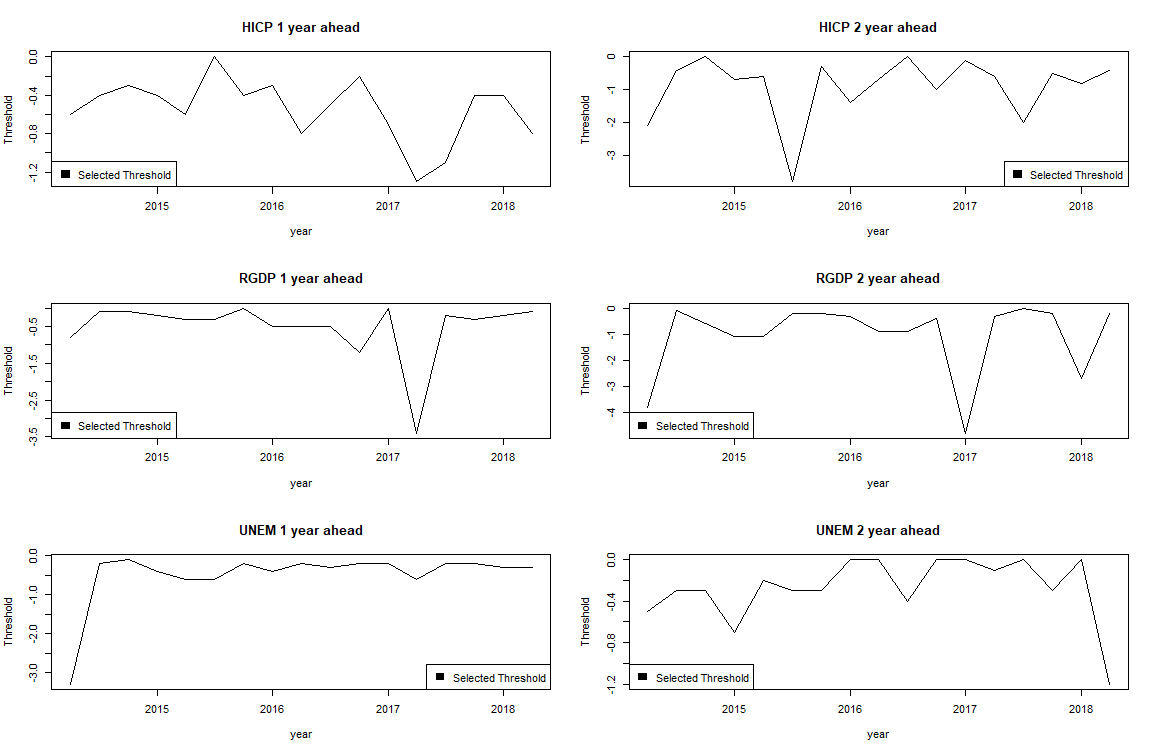
\includegraphics{./Images/Fluctuation.pdf}
		\caption{Truncation selections for different OOS periods}\label{fig: fluctuation}
	\end{figure}
	
	\subsection{Bias weighting}\label{bias-weighting}
	
	Bias weighting produces an interesting case here. If the bias estimation model estimates the predictable part and the unpredictable error successfully, this success can be attributed to better weight selection through the additional information. Our approach to bias estimation is similar to \cite{Gibbs2017} but deviates in the variable used. We estimate the bias by
	\begin{equation}
	\label{eqn: bias estimation}
	\epsilon_{i,t} = \alpha + \gamma_i y_{i,t} + \eta_{i,t}
	\end{equation}
	We then produce the estimated future forecast bias by taking the expected value
	\begin{equation}
	E(\epsilon_{i,t+1}) = \alpha + \gamma_i y_{i,t+1}.
	\end{equation}
	\citeauthor{Gibbs2017} uses true macroeconomic data, while we use the forecast itself. Essentially, they are interchangeable. Rewrite Equation \ref{eqn: bias estimation} as
	\begin{equation}
	\begin{aligned}
	\epsilon_{i,t} &= \frac{\alpha}{1+\gamma_i}+\frac{\gamma_i}{1+\gamma_i}y_t + \frac{1}{1+\gamma_i}\eta_{i,t}\\
	&= \alpha^* + \gamma_i^* y_t + \eta_{i,t}^*,
	\end{aligned} 
	\end{equation}
	and equation \ref{eqn: bias estimation} becomes the equation given by \citeauthor{Gibbs2017}.
	
	Tables \ref{tab: MSPE HICP bias}, \ref{tab: MSPE RGDP bias}, and \ref{tab: MSPE UNEM bias} show the effect of truncation with a bias-corrected weight. The estimation of the bias increases the estimation error, creating another trade-off between the estimation error and the bias. Only two out of six scenarios have produced a ratio below 1, producing considerably worse results than those produced without bias correction. The two scenarios are RGDP with a two-year horizon and UNEM with a one-year horizon, with minimum ratios of 0.83 and 0.56, respectively. For HICP with bias correction, the truncation performs best with the highest threshold at zero. This result differs from that of no-bias selection, where the best threshold is achieved below zero.
	
	\begin{table}[!h]
		\centering
		\caption{Mean Squared Prediction Error (MSPE) and Mean Absolute Prediction Error (MAPE) ratios for bias-corrected inflation for various truncation values.}
		\label{tab: MSPE HICP bias}
		\begin{tabular}{lcccc}
			\hline
			&                        \multicolumn{4}{c}{HICP}                         \\
			\cmidrule(lr){2-5}                              & \multicolumn{2}{c}{one year Horizon} & \multicolumn{2}{c}{two years Horizon} \\
			\cmidrule(lr){2-3} \cmidrule(lr){4-5}
			Threshold & MSPE Ratio & MAPE Ratio  & MSPE Ratio & MAPE Ratio  \\ \hline
			-$\infty$ & 2.7747 & 1.7760 & 1.6452 & 1.3735\\ 
			-5 & 2.7747 & 1.7760 & 1.6452 & 1.3735\\ 
			-4.5 & 2.7747 & 1.7760 & 1.6452 & 1.3735\\ 
			-4 & 2.7747 & 1.7760 & 1.6452 & 1.3735\\ 
			-3.5 & 2.7747 & 1.7760 & 1.6452 & 1.3735\\ 
			-3 & 2.7747 & 1.7760 & 1.5888 & 1.2976\\ 
			-2.5 & 2.7747 & 1.7760 & 1.6059 & 1.3276\\ 
			-2 & 2.7747 & 1.7760 & 1.5955 & 1.3064\\ 
			-1.5 & 2.7747 & 1.7760 & 1.5887 & 1.2871\\ 
			-1 & 2.6528 & 1.6894 & 1.1640 & 1.1141\\ 
			-0.5 & 1.7696 & 1.3260 & 1.0464 & 1.0365\\ 
			0 & 1.1118 & 1.0576 & 1.0221 & 1.0231\\ \hline
		\end{tabular}
	\end{table}
	
	
	RGDP shows similar results for the one-year horizon, where truncation helps, but selecting 0 as the threshold produces the best performance. On the other hand, RGDP with a two-year horizon is able to achieve an MSPE ratio of 0.83 with a truncation value of -1. The selection for the MAPE ratio yields the same truncation. Comparing this to RGDP without a bias correction, the bias-corrected forecast performs worse for the one-year horizon, but performs better for the two-year horizon. The best truncations result from a truncation value of -1.5 for the one-year horizon and 0 for the two-year horizon with no correction to 0 and -1, respectively.
	
	\begin{table}[!h]
		\centering
		\caption{Mean Squared Prediction Error (MSPE) and Mean Absolute Prediction Error (MAPE) ratios for bias-corrected economic growth for various truncation values.}
		\label{tab: MSPE RGDP bias}
		\begin{tabular}{lcccc}
			\hline
			&                        \multicolumn{4}{c}{RGDP}                         \\
			\cmidrule(lr){2-5}                              & \multicolumn{2}{c}{one year Horizon} & \multicolumn{2}{c}{two years Horizon} \\
			\cmidrule(lr){2-3} \cmidrule(lr){4-5}
			Threshold & MSPE Ratio & MAPE Ratio  & MSPE Ratio & MAPE Ratio  \\ \hline
			-$\infty$ & 3.3002 & 1.5457 & 1.0535 & 0.9458\\ 
			-5 & 1.7581 & 1.2626 & 1.1094 & 0.9846\\ 
			-4.5 & 1.7915 & 1.2894 & 1.1094 & 0.9846\\ 
			-4 & 1.7910 & 1.2888 & 1.1069 & 0.9833\\ 
			-3.5 & 1.8086 & 1.298 & 1.1079 & 0.9838\\ 
			-3 & 1.8101 & 1.2984 & 1.1076 & 0.9837\\ 
			-2.5 & 1.8118 & 1.3004 & 1.0691 & 0.9716\\ 
			-2 & 1.6089 & 1.3075 & 0.9950 & 0.9438\\ 
			-1.5 & 1.4604 & 1.2530 & 0.8630 & 0.8931\\ 
			-1 & 1.2764 & 1.1320 & 0.8275 & 0.8753\\ 
			-0.5 & 1.0758 & 1.0464 & 0.9437 & 0.9508\\ 
			0 & 1.0436 & 1.0264 & 0.9835 & 0.9892\\ \hline
		\end{tabular}
	\end{table}
	
	
	The UNEM one-year horizon has ratios as low as 0.56, which is a large improvement over the equal- weights case. However, this effect is not duplicated for the two-year horizon. The two-year horizon's MSPE ratios are higher than those for equal weights.
	
	
	\begin{table}[!h]
		\centering
		\caption{Mean Squared Prediction Error (MSPE) and Mean Absolute Prediction Error (MAPE) ratios for bias-corrected unemployment for various truncation values.}
		\label{tab: MSPE UNEM bias}
		\begin{tabular}{lcccc}
			\hline
			&                        \multicolumn{4}{c}{UNEM}                         \\
			\cmidrule(lr){2-5}                              & \multicolumn{2}{c}{one year Horizon} & \multicolumn{2}{c}{two years Horizon} \\
			\cmidrule(lr){2-3} \cmidrule(lr){4-5}
			Threshold & MSPE Ratio & MAPE Ratio  & MSPE Ratio & MAPE Ratio  \\ \hline
			-$\infty$ & 3.7993 & 1.4829 & 21.2312 & 3.0358\\ 
			-5 & 3.7993 & 1.4829 & 2.5172 & 1.5149\\ 
			-4.5 & 3.7993 & 1.4829 & 2.5172 & 1.5149\\ 
			-4 & 3.7993 & 1.4829 & 2.5376 & 1.5293\\ 
			-3.5 & 3.7993 & 1.4829 & 2.5287 & 1.5246\\ 
			-3 & 3.3185 & 1.3959 & 2.3569 & 1.4439\\ 
			-2.5 & 2.3783 & 1.1662 & 2.3491 & 1.4493\\ 
			-2 & 0.9828 & 0.8032 & 2.3203 & 1.4382\\ 
			-1.5 & 0.7950 & 0.7275 & 1.6368 & 1.2530\\ 
			-1 & 0.5564 & 0.6864 & 1.3372 & 1.1226\\ 
			-0.5 & 0.7253 & 0.8155 & 1.1141 & 1.0643\\ 
			0 & 0.8736 & 0.9201 & 1.0327 & 1.0176\\ \hline
		\end{tabular}
	\end{table}
	
	Figure \ref{fig: Ratio bias} shows the MSPE and MAPE ratios plotted against the threshold values with higher granularity. HICP does not show to reach the minimum with thresholds of up to 0 for both forecast horizons. The same conclusion holds for RGDP with a one-year horizon and UNEM with a two-year horizon. On the other hand, RGDP with a two-year horizon exhibits a large effect on truncation when bias correction is used and performs badly without bias correction. One reason for this result is that RGDP is highly biased over time,  a situation which cannot be corrected using cross-sectional truncation. UNEM with a one-year horizon is another macroeconomic topic that performs better with bias correction. We see from its plot that a large portion of the curve is well below 0.7, eliminating the problem of selecting -0.5 precisely.
	
	
	\begin{figure}[!h]
		\centering
		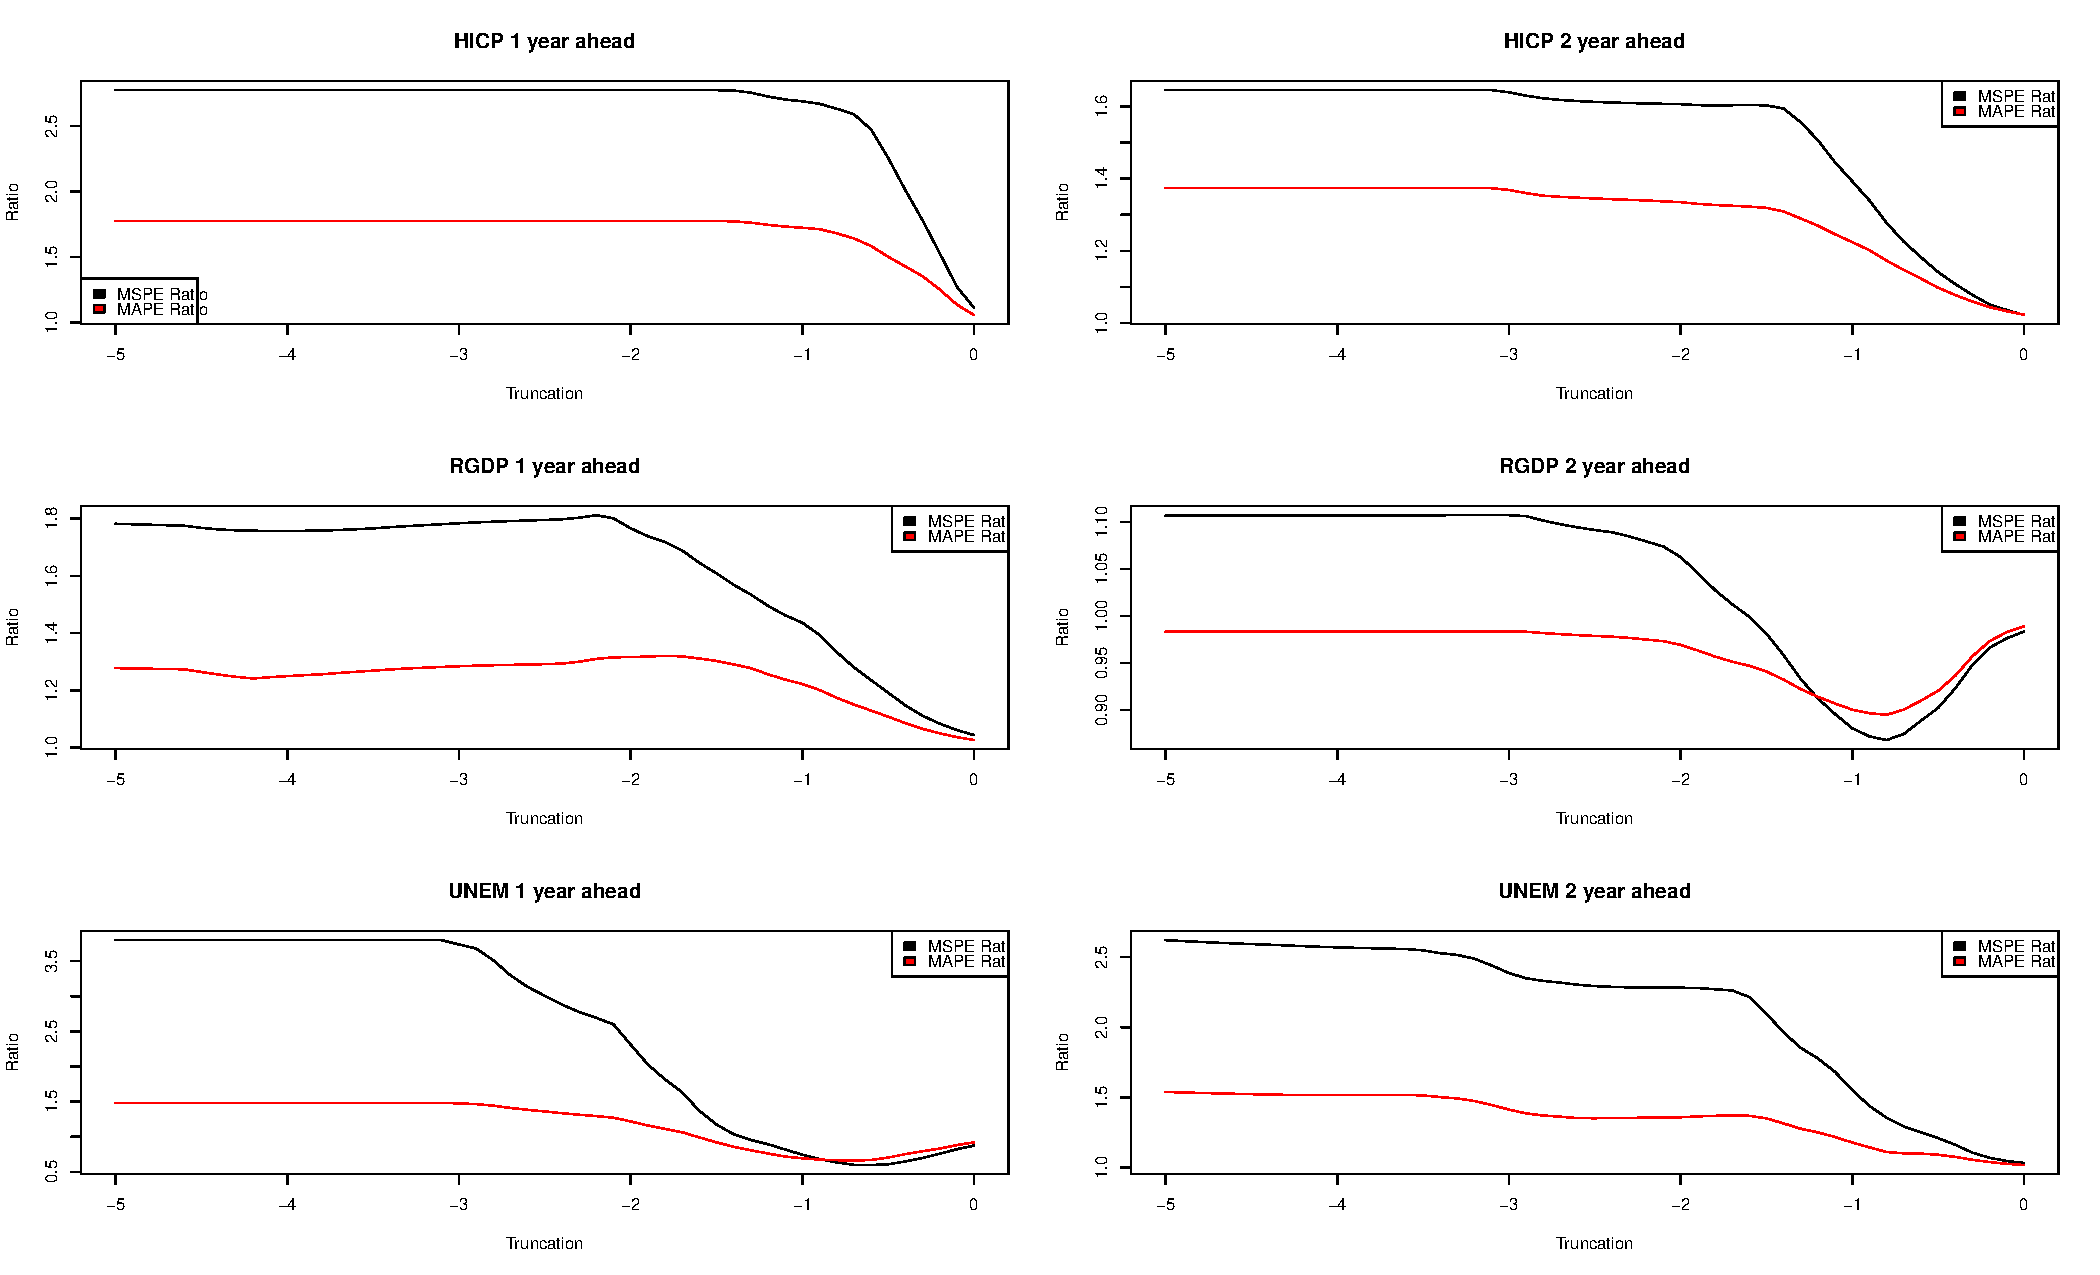
\includegraphics{./Images/Ratio_c_bias.pdf}
		\caption{MSPE Ratio for different macroeconomic topics with bias correction}\label{fig: Ratio bias}
	\end{figure}
	
	
	\begin{figure}[!h]
		\centering
		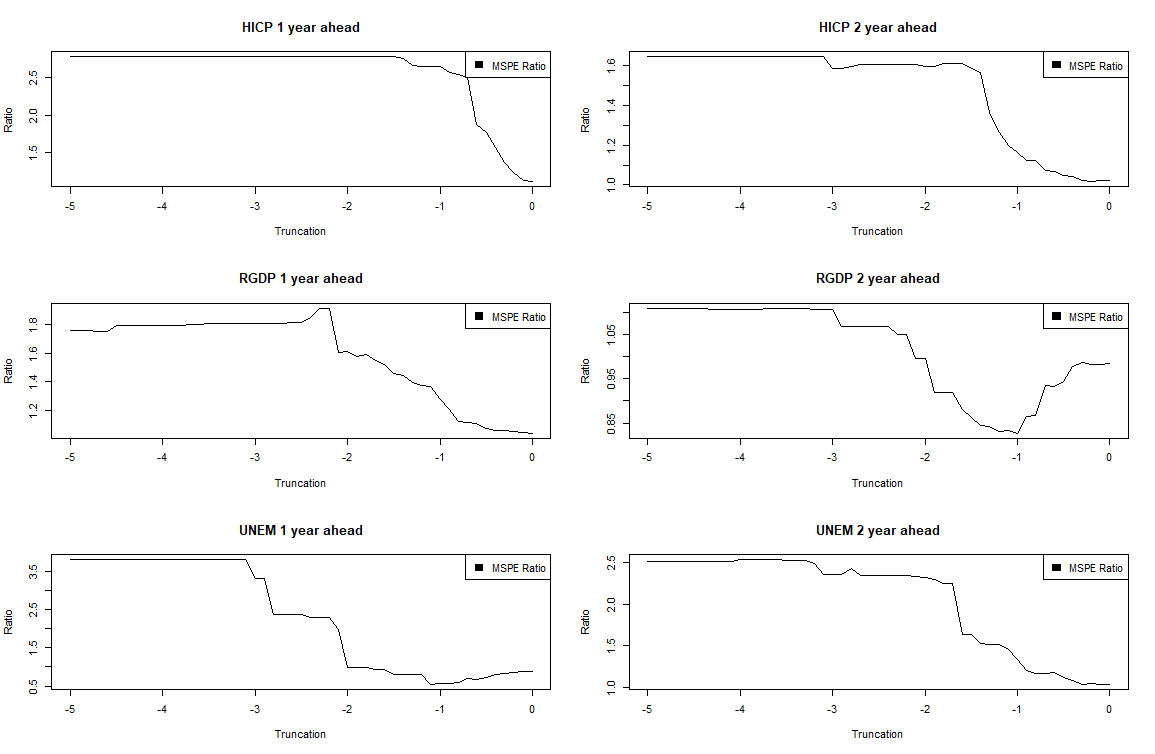
\includegraphics{./Images/Ratio Bias.pdf}
		\caption{MSPE ratios for different macroeconomic topics with bias correction}\label{fig: Ratio bias}
	\end{figure}
	
	
	All in all, we have examined the possibility of combining bias correction and truncation. Some macroeconomic topics perform better with the only truncation, while some perform better with the addition of bias correction. A possible explanation for these differences is that the truncation has effect in a different direction than the bias correction. Truncation relies on the high correlation between different $y_i$, while bias-correction relies on the consistency and predictability of the forecast error in a univariate setting. This difference between the two approaches explains the different effects on the series. If the predictability of the forecast error is small, i.e., predicting the forecast increases the MSE, adjusting the bias does not help. Of course, truncation and bias correction are not mutually independent. An increase in the correlation increases the similarity of the estimation error. In turn, the estimation errors do not cancel out but magnify instead. 
	
	
	
	\subsection{Simulation}\label{simulation}
	In this section, we show a different effect of the underlying model's influence the MSPE. For simplicity, we select four true weights and change the data-generating model with regards to the correlations and error variance. We start with true weight $w=(-0.5,0.3,0,1.2)'$ and proceed with a correlation matrix in which all of the off-diagonals have the same value. The covariance matrix follows by setting all variances equal to 1. The error term is generated with a univariate random normal distribution, while the forecasts are generated by the multivariate normal distribution. We will not use biased forecasts in this simulation. The simulation runs 10 observations per simulation for a total of 2000 runs for each correlation and error variance combination. Then the simulation takes the average of the MSPEs obtained.
	
	In Figure \ref{fig: simulation}, the different effects of the correlations and error variances are shown. We select four different correlations, from 0.5 to 0.8, covering most of the correlations we observed in the SPF. For the error variances, the selection ranges from 0.4 to 0.9. Since the variance of the data is 1, each error variance quickly gives an idea of the fit of its forecast. 
	
	When examining Figure \ref{fig: simulation}, changes in the correlation and error variance do not influence where the MSPE drops or rises. Changes in the error variance influence the level of the MSPE trivially. A higher error variance leads to a higher MSPE. Changes in the correlation show where the truncation effect converges to. For low correlations, 0.5 and 0.6, there is a distinct upward movement when the truncation goes to 0 for all error variances. This forms the U-shape one expects when the bias increases. For a high correlation, the truncation effect does not increase the bias enough, making the U-shape observable in only a few cases. Other cases with higher error variances show a continuous decline in the MSPE. 
	
	Referring back to Section \ref{bias-weighting}, the changes in the shape can be accounted for by the additional estimation error caused by the bias term. Considering Figure \ref{fig: simulation}, similar plots could be obtained for a correlation of 0.7 and the error variance going from 0.7 to 0.9.
	
	For a U-shape to exist, e.g., equal weights are not the best forecasting technique, the correlations and error variances both play important roles. A higher correlation only allows a lower error when finding the optimal truncation parameter, while a lower correlation allows a higher error to exist.
	
	\begin{figure}[!h]
		\centering
		\includegraphics{./Images/Simulation2.pdf}
		\caption{MSPE for different correlations and error variances.}\label{fig: simulation}
	\end{figure}
	
	\section{Conclusion and discussion}\label{conclusion}
	In this paper, we looked into the possibility of using truncation to improve forecasts within a forecast combination. A simple weight derived with a deterministic weight assumption often exhibits poor empirical behaviour when compared to the equal weights achieved via the arithmetic mean. Equal weights produce a behaviour that the combined forecast has to be between the minimum and the maximum of all forecast. This limitation also holds for all any weight selection method in which the weight cannot be negative. 
	
	Using truncation, five out of six macroeconomic scenarios have a positive effect on the MSPE and MAPE for the ECB's SPF. The survey forecasts are strongly correlated, and the true values they are predicting often lie outside of the minimum/maximum range of the forecasts. Additionally, the high correlations lead to an increase in the negative weight. Therefore, the relaxation of the no-negative-weight restriction helps in this aspect.
	
	When engaging in truncation, we also set the weight below a certain threshold to 0, which removes the forecasts tied to these weights from the combination list. The results indicate a positive effect, with up to a 30\% decrease in the MSPE compared to the value obtained in the case of equal weights. This is positive news considering that the number of forecasters is relatively large compared to the sample size. With up to 120 forecasters and 60 observations, the weight estimation contains a large amount of estimation noise. This noise allows the estimated weight to vary widely from -21.79 to 16.34. On the other hand, the weights calculated via the equal weight method are around 0.01.
	
	The effect of truncation comes into play when the optimal threshold selection for the underlying truncation parameter is used. The MSPE can be decreased by between 12\% and 30\%. Using an optimal threshold provides room for variation in the parameters over time, as opposed to situations in which the parameters remain constant. hence, this process leads to a performance increase for RGDP with a two-year forecasting horizon. Improvements in the MAPE and MSPE ratios are noted for all 6 microeconomic scenarios when compared to the values obtained using equal weights. A majority of the parameters are under -1.5 for the chosen truncation. Of course, this is well under the initial -21.79. Variation is limited by requiring the parameters to be under -1.5, thus reducing the estimation error and variance. 
	
	Looking into the weight selection further, it is possible that the SPF is dominated by the consistent bias of a certain forecaster. As an example, suppose that a certain forecaster undervalues growth and decline, resulting in a forecast closer to 0 than the true value. When we construct the bias-correcting forecast weight and apply the truncation analysis to the corrected weight, the result is a mixed bag of good and bad news. Four out of six macroeconomic scenarios are worse than what would have been obtained using equal weights, while, without bias correction, we have only one truncation weight that is underperforming. The test statistics decrease compared to the non-truncated test statistics. Bias correction improves the only macro topic forecasts that do not outperform equal-weight forecasts without bias correction. The MSPE ratio decreases up to 17\% compared with the equal-weight case, and the MAPE ratio decreases up to 12 \%. Further, there is an additional decrease of 13\% in the UNEM for the one-year horizon. The difference between with and without bias correction could go in the direction of the changes in the weight. Truncation tries to extend the forecast range by using a negative weight, while bias correction tries to identify the consistent bias within each forecaster.
	
	We also studied the different effects of correlation and estimation uncertainty on the shape of the MSPE. Correlation and estimation uncertainty both play important and intertwined roles in the truncation. A higher correlation only results in a lower error when finding the optimal truncation parameter, while a lower correlation allows a higher error to exist. Since estimation uncertainty and correlations can be known before applying the truncation, the selection of the best truncation using that information is a possible future research topic.
	
	We list a few other points in this paper that require further research. All analytic derivations were done using two-forecast scenarios, and this process can be extended to the multivariate setting. RGDP with a two-year horizon exhibited an unexpected shape of for the plot of the MSPE again the truncation values, but the reason for this shape remains unclear. Knowing the reason for the spikes during truncation selection is helpful, as it can limit variation - a combination of other techniques, such as shrinking the covariance, could be used to improve the estimates. Additionally, using a threshold value other than 0 for the truncation could also change the effects of the method.
	
	All in all, we demonstrated that truncation could improve upon equal weights. Means for improvement lie in the correlations and forecasting uncertainty. When the conditions are met, for example, in the SPF data, equal weights is no longer the prime choice for the forecast combination. 
	
	\newpage
	
	\bibliographystyle{apalike}
	\bibliography{shortbib}
	
\end{document}


